\documentclass[10pt,a4paper,oneside]{article}
\usepackage[utf8]{inputenc}
\usepackage[english]{babel}
\usepackage{forloop}
\usepackage{amsmath}
\usepackage{amsfonts}
\usepackage{amssymb}
\usepackage{gensymb}
\usepackage{graphicx}
\usepackage[dvipsnames]{xcolor}
\usepackage{tikz}
\usetikzlibrary{arrows,automata,shapes}
\tikzstyle{decision} = [diamond, draw, fill=blue!20, text width=4.5em, text badly centered, node distance=2.5cm, inner sep=0pt]
\tikzstyle{block} = [rectangle, draw, fill=blue!20, text width=5em, text centered, rounded corners, minimum height=4em]
\tikzstyle{line} = [draw, very thick, color=black!50, -latex']
\tikzstyle{cloud} = [draw, ellipse,fill=red!20, node distance=2.5cm,minimum height=2em]
\usepackage[siunitx]{circuitikz}

\definecolor{LightGray}{gray}{0.9}
\definecolor{NormalGray}{gray}{0.8}
\definecolor{DarkGray}{gray}{0.7}
\definecolor{DarkDarkGray}{gray}{0.5}

\usepackage[colorlinks=true,linkcolor=blue,urlcolor=black,bookmarksopen=true]{hyperref}
\usepackage{bookmark}
\usepackage{hyperref}
\usepackage{sepfootnotes}

\usepackage[srcmeas]{circdia}

\title{Libre Silicon process specification}
\date{\today} 
\author{David Lanzendörfer}
\makeindex

\begin{document}
\maketitle

\begin{abstract}
	Copyright © 2017 LANCEVILLE TECHNOLOGY GROUP CO., LIMITED. All rights reserved. \\

	This process is licensed under the Libre Silicon public license; you can redistribute it and/or modify it under the terms of the Libre Silicon public license
	as published by the Libre Silicon alliance, either version 1 of the License, or (at your option) any later version.

	This design is distributed in the hope that it will be useful, but WITHOUT ANY WARRANTY; without even the implied warranty of MERCHANTABILITY or FITNESS FOR A PARTICULAR PURPOSE.
	See the Libre Silicon Public License for more details. \\

	This is the specification of the free silicon manufacturing standard for manufacturing the LibreSilicon standard logic cells\footnote{https://github.com/chipforge/StdCellLib} and related free technology nodes from the LibreSilicon project.
\end{abstract}

\newpage
\tableofcontents
\newpage
\section{CMOS in a nutshell}
This basic initial project is dedicated to the CMOS Technology only and for this reason two types of metal–oxide–semiconductor field-effect transistors (MOSFET) are required.

Historicaly, the first chips with MOSFETs on the mass market were p-channel MOSFETs in enhancement-mode.

\begin{center}
	\begin{figure}[h]
		\begin{center}
			\begin{circuitdiagram}{20}{20}
				\power{15}{18.5}{U}{}  % power above pmos
				\wire{15}{18}{15}{16}   % wire above pmos
				\trans{penh}{13}{14}{R}{}{} % pmos -> right
				\Voltarrow{14}{18}{10}{16}{u}{$-V_{GS}$}
				\wire{15}{12}{15}{8}   % wire below pmos
				\resis{15}{5}{V}{$R_D$}{}  % resistor on drain
				\wire{15}{1}{15}{2}   % wire below pmos
				\ground{15}{0.5}{D}  % ground below resistor
				\othersrc[\sigsym{-rec}]{o}{5.5}{15.5}{H}{}{signal}
				\pin{9.5}{15.5}{R}{}	% pin in
				\ground{2.5}{0.5}{D}  % ground below signal source
				\wire{2.5}{1}{2.5}{15.5}   % wire below signal
				\junct{15}{10}   % dot
				\wire{15}{10}{16}{10}   % wire before out
				\pin{17}{10}{R}{out}	% pin out
			\end{circuitdiagram}
		\end{center}
		\caption{enhancement-mode PMOS transistor use-case}
	\end{figure}
\end{center}

The sectional view of a PMOS transistor in silicon is being shown below
\begin{center}
	\begin{figure}[h]
		\begin{center}
			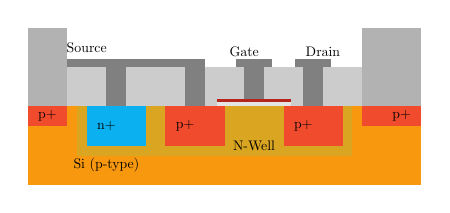
\begin{tikzpicture}[node distance = 3cm, auto, thick,scale=0.5, every node/.style={transform shape}]
				% substrate
				\fill[YellowOrange] (0,0) rectangle (10,2);
				\node at (2,0.5) {Si (p-type)};

				% n-well
				\fill[Goldenrod] (1.25,0.75) rectangle (8.25,2);
				\node at (5.75,1) {N-Well};

				% body
				\fill[ProcessBlue] (1.5,1) rectangle (3,2);
				\node at (2,1.5) {n+};
				% source
				\fill[RedOrange] (3.5,1) rectangle (5,2);
				\node at (4,1.5) {p+};
				% drain
				\fill[RedOrange] (6.5,1) rectangle (8,2);
				\node at (7,1.5) {p+};
				%% gate:
				% gate oxide
				\fill[LightGray] (4.8,2) rectangle (6.7,2.1);
				% gate poly
				\fill[BrickRed] (4.8,2.1) rectangle (6.7,2.2);

				% metals ground
				\fill[DarkDarkGray] (2,2) rectangle (2.5,3);
				\fill[DarkDarkGray] (4,2) rectangle (4.5,3);
				\fill[DarkDarkGray] (1,3) rectangle (4.5,3.2); % connection pad GND

				\fill[DarkDarkGray] (5.5,2.2) rectangle (6,3);
				\fill[DarkDarkGray] (5.3,3) rectangle (6.2,3.2); % connection pad VG

				\fill[DarkDarkGray] (7,2) rectangle (7.5,3);
				\fill[DarkDarkGray] (6.8,3) rectangle (7.7,3.2); % connection pad VDD

				% isolation oxides:
				\fill[NormalGray] (1,2) rectangle (2,3);
				\fill[NormalGray] (2.5,2) rectangle (4,3);
				\fill[NormalGray] (4.5,2) rectangle (4.8,3);
				\fill[NormalGray] (4.8,2.2) rectangle (5.5,3);
				\fill[NormalGray] (6,2.2) rectangle (6.7,3);
				\fill[NormalGray] (6.7,2) rectangle (7,3);
				\fill[NormalGray] (7.5,2) rectangle (8.5,3);

				\node at (1.5,3.5) {Source};
				\node at (5.5,3.4) {Gate};
				\node at (7.5,3.4) {Drain};

				%field oxides:
				\fill[DarkGray] (0,2) rectangle (1,4);
				\fill[DarkGray] (8.5,2) rectangle (10,4);
				\fill[RedOrange] (0,1.5) rectangle (1,2);
				\node at (0.5,1.75) {p+};
				\fill[RedOrange] (8.5,1.5) rectangle (10,2);
				\node at (9.5,1.75) {p+};
			\end{tikzpicture}
		\end{center}
		\caption{Sectional view of a PMOS transistor}
	\end{figure}
\end{center}

Historicaly later, faster chips with MOSFETs on the mass market were marked as n-channel MOSFETs in enhancement mode also.

\begin{center}
	\begin{figure}[h]
		\begin{center}
			\begin{circuitdiagram}{20}{20}
				\power{15}{18.5}{U}{}  % power above resistor
				\wire{15}{17}{15}{18}   % wire above resistor
				\resis{15}{14}{V}{$R_D$}{}  % resistor on drain
				\wire{15}{11}{15}{8}   % wire between resistor and nmos
				\trans{nenh}{13}{6}{R}{}{} % nmos -> right
				\Voltarrow{10}{4}{14}{1}{d}{$+V_{GS}$}
				\wire{15}{1}{15}{4}   % wire below nmos
				\ground{15}{0.5}{D}  % ground below nmos
				\othersrc[\sigsym{rec}]{o}{5.5}{4.5}{H}{}{signal}
				\pin{9.5}{4.5}{R}{}	% pin in
				\ground{2.5}{0.5}{D}  % ground below signal source
				\wire{2.5}{1}{2.5}{4.5}   % wire below signal
				\junct{15}{10}   % dot
				\wire{15}{10}{16}{10}   % wire before out
				\pin{17}{10}{R}{out}	% pin out
			\end{circuitdiagram}
		\end{center}
		\caption{enhancement-mode NMOS transistor use-case}
	\end{figure}
\end{center}

The sectional view of a NMOS transistor in silicon is being shown here also.
\begin{center}
	\begin{figure}[h]
		\begin{center}
			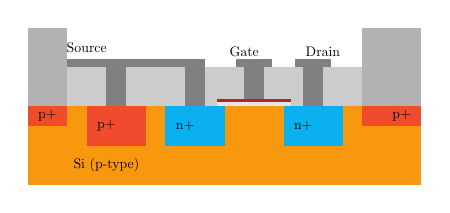
\begin{tikzpicture}[node distance = 3cm, auto, thick,scale=0.5, every node/.style={transform shape}]
				% substrate
				\fill[YellowOrange] (0,0) rectangle (10,2);
				\node at (2,0.5) {Si (p-type)};
				% body
				\fill[RedOrange] (1.5,1) rectangle (3,2);
				\node at (2,1.5) {p+};
				% source
				\fill[ProcessBlue] (3.5,1) rectangle (5,2);
				\node at (4,1.5) {n+};
				% drain
				\fill[ProcessBlue] (6.5,1) rectangle (8,2);
				\node at (7,1.5) {n+};
				%% gate:
				% gate oxide
				\fill[LightGray] (4.8,2) rectangle (6.7,2.1);
				% gate poly
				\fill[BrickRed] (4.8,2.1) rectangle (6.7,2.2);
				% metals ground
				\fill[DarkDarkGray] (2,2) rectangle (2.5,3);
				\fill[DarkDarkGray] (4,2) rectangle (4.5,3);
				\fill[DarkDarkGray] (1,3) rectangle (4.5,3.2); % connection pad GND

				\fill[DarkDarkGray] (5.5,2.2) rectangle (6,3);
				\fill[DarkDarkGray] (5.3,3) rectangle (6.2,3.2); % connection pad VG

				\fill[DarkDarkGray] (7,2) rectangle (7.5,3);
				\fill[DarkDarkGray] (6.8,3) rectangle (7.7,3.2); % connection pad VDD

				% isolation oxides:
				\fill[NormalGray] (1,2) rectangle (2,3);
				\fill[NormalGray] (2.5,2) rectangle (4,3);
				\fill[NormalGray] (4.5,2) rectangle (4.8,3);
				\fill[NormalGray] (4.8,2.2) rectangle (5.5,3);
				\fill[NormalGray] (6,2.2) rectangle (6.7,3);
				\fill[NormalGray] (6.7,2) rectangle (7,3);
				\fill[NormalGray] (7.5,2) rectangle (8.5,3);

				%field oxides:
				\fill[DarkGray] (0,2) rectangle (1,4);
				\fill[DarkGray] (8.5,2) rectangle (10,4);
				\fill[RedOrange] (0,1.5) rectangle (1,2);
				\node at (0.5,1.75) {p+};
				\fill[RedOrange] (8.5,1.5) rectangle (10,2);
				\node at (9.5,1.75) {p+};

				\node at (1.5,3.5) {Source};
				\node at (5.5,3.4) {Gate};
				\node at (7.5,3.4) {Drain};
			\end{tikzpicture}
		\end{center}
		\caption{Sectional view of a NMOS transistor}
	\end{figure}
\end{center}

Both technologies, the older NMOS as the newer PMOS, have the same disadvantage. Every time, the transistor is switched on, the current between Drain and Source of the transistor is limited by the Resistor on Drain only. Higher currents here meaning also higher power consumption for the chip where the transistors are integrated also. If the transistors are switched off, now currents flows between Drain and Source anymore, the power consumption of the chip also goes low.
Et violà, the US-Patent with Number 3356858\footnote{https://www.google.com/patents/US3356858} changed the world and combines both technologies to the new complementary metal-oxide-semiconductor (CMOS) technology. Instead of every transistor is working against a weak resistor, the transistor works against a complementary switched-off transistor. With the Eyes of our antecessor CMOS doubles the transistor count, but contemporary chips all are build in CMOS.

\begin{center}
	\begin{figure}[h]
		\begin{center}
			\begin{circuitdiagram}{20}{20}
				\power{15}{18.5}{U}{}  % power above pmos 
				\wire{15}{16}{15}{18}   % wire above pmos
				\trans{penh}{13}{14}{R}{}{} % pmos -> right
				\Voltarrow{14}{18}{10}{16}{u}{$-V_{GS}$}
				\wire{15}{8}{15}{12}   % wire between pmos and nmos
				\trans{nenh}{13}{6}{R}{}{} % nmos -> right
				\Voltarrow{10}{4}{14}{1}{d}{$+V_{GS}$}
				\wire{15}{1}{15}{4}   % wire below nmos
				\ground{15}{0.5}{D}  % ground below nmos
				\othersrc[\sigsym{rec}]{o}{5}{10}{H}{}{signal}
				\pin{9}{10}{R}{}	% pin in
				\wire{9.5}{10}{10}{10}   % wire before gates
				\wire{10}{15.5}{10}{4.5}   % wire between gates
				\junct{10}{10}   % dot
				\ground{2}{0.5}{D}  % ground below signal source
				\wire{2}{1}{2}{10}   % wire below signal
				\junct{15}{10}   % dot
				\wire{15}{10}{16}{10}   % wire before out
				\pin{17}{10}{R}{out}	% pin out
			\end{circuitdiagram}
		\end{center}
		\caption{complementary PMOS and NMOS transistor couple use-case}
	\end{figure}
\end{center}

Below the sectional view of the inverter circuitry can be seen.
For the run through of this process we will use this cross section diagram as reference.
\begin{center}
	\begin{figure}[h]
		\begin{center}
			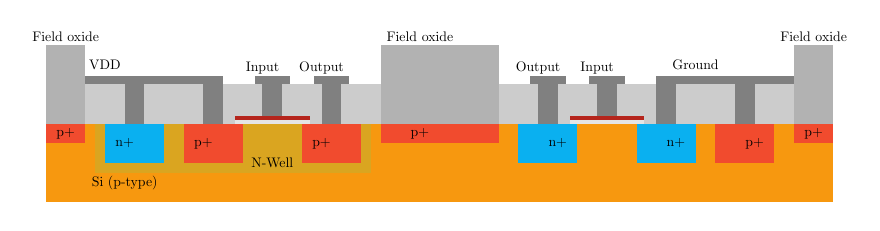
\begin{tikzpicture}[node distance = 3cm, auto, thick,scale=0.5, every node/.style={transform shape}]
				% substrate
				\fill[YellowOrange] (0,0) rectangle (20,2);
				\node at (2,0.5) {Si (p-type)};
				% n-well
				\fill[Goldenrod] (1.25,0.75) rectangle (8.25,2);
				\node at (5.75,1) {N-Well};
				% body
				\fill[ProcessBlue] (1.5,1) rectangle (3,2);
				\node at (2,1.5) {n+};
				% source
				\fill[RedOrange] (3.5,1) rectangle (5,2);
				\node at (4,1.5) {p+};
				% drain
				\fill[RedOrange] (6.5,1) rectangle (8,2);
				\node at (7,1.5) {p+};
				%% gate:
				% gate oxide
				\fill[LightGray] (4.8,2) rectangle (6.7,2.1);
				% gate poly
				\fill[BrickRed] (4.8,2.1) rectangle (6.7,2.2);
				% isolation oxides:
				\fill[NormalGray] (1,2) rectangle (2,3);
				\fill[NormalGray] (2.5,2) rectangle (4,3);
				\fill[NormalGray] (4.5,2) rectangle (4.8,3);
				\fill[NormalGray] (4.8,2.2) rectangle (5.5,3);
				\fill[NormalGray] (6,2.2) rectangle (6.7,3);
				\fill[NormalGray] (6.7,2) rectangle (7,3);
				\fill[NormalGray] (7.5,2) rectangle (8.5,3);

				%field oxides:
				\fill[DarkGray] (0,2) rectangle (1,4);
				\fill[DarkGray] (8.5,2) rectangle (11.5,4);
				\fill[DarkGray] (19,2) rectangle (20,4);

				\fill[RedOrange] (0,1.5) rectangle (1,2);
				\fill[RedOrange] (8.5,1.5) rectangle (11.5,2);
				\fill[RedOrange] (19,1.5) rectangle (20,2);

				\node at (0.5,1.75) {p+};
				\node at (9.5,1.75) {p+};
				\node at (19.5,1.75) {p+};

				%%% nmos:
				% body
				\fill[RedOrange] (17,1) rectangle (18.5,2);
				\node at (18,1.5) {p+};
				% source
				\fill[ProcessBlue] (15,1) rectangle (16.5,2);
				\node at (16,1.5) {n+};
				% drain
				\fill[ProcessBlue] (12,1) rectangle (13.5,2);
				\node at (13,1.5) {n+};

				%% gate:
				% gate oxide
				\fill[LightGray] (13.3,2) rectangle (15.2,2.1);
				% gate poly
				\fill[BrickRed] (13.3,2.1) rectangle (15.2,2.2);

				% metals
				\fill[DarkDarkGray] (17.5,2) rectangle (18,3);
				\fill[DarkDarkGray] (15.5,2) rectangle (16,3);
				\fill[DarkDarkGray] (15.5,3) rectangle (19,3.2); % connection pad GND

				\fill[DarkDarkGray] (14,2.2) rectangle (14.5,3);
				\fill[DarkDarkGray] (13.8,3) rectangle (14.7,3.2); % connection pad VG

				\fill[DarkDarkGray] (12.5,2) rectangle (13,3);
				\fill[DarkDarkGray] (12.3,3) rectangle (13.2,3.2); % connection pad VDD

				\fill[DarkDarkGray] (2,2) rectangle (2.5,3);
				\fill[DarkDarkGray] (4,2) rectangle (4.5,3);
				\fill[DarkDarkGray] (1,3) rectangle (4.5,3.2); % connection pad GND

				\fill[DarkDarkGray] (5.5,2.2) rectangle (6,3);
				\fill[DarkDarkGray] (5.3,3) rectangle (6.2,3.2); % connection pad VG

				\fill[DarkDarkGray] (7,2) rectangle (7.5,3);
				\fill[DarkDarkGray] (6.8,3) rectangle (7.7,3.2); % connection pad VDD

				% isolation oxides:
				\fill[NormalGray] (18,2) rectangle (19,3);
				\fill[NormalGray] (16,2) rectangle (17.5,3);
				\fill[NormalGray] (15.2,2) rectangle (15.5,3);
				\fill[NormalGray] (14.5,2.2) rectangle (15.2,3);
				\fill[NormalGray] (13.3,2.2) rectangle (14,3);
				\fill[NormalGray] (13,2) rectangle (13.3,3);
				\fill[NormalGray] (11.5,2) rectangle (12.5,3);

				\node at (1.5,3.5) {VDD};
				\node at (16.5,3.5) {Ground};
				\node at (5.5,3.4) {Input};
				\node at (14,3.4) {Input};
				\node at (7,3.4) {Output};
				\node at (12.5,3.4) {Output};

				\node at (0.5,4.2) {Field oxide};
				\node at (9.5,4.2) {Field oxide};
				\node at (19.5,4.2) {Field oxide};
			\end{tikzpicture}
		\end{center}
		\caption{Sectional view of a NMOS-PMOS transistor circuit}
	\end{figure}
\end{center}

\newpage
\section{Physics}
\subsection{Infusion}
The redistribution process depends on the ratio of the solubility of the doping material in silicon and SiO$ _2$. At the Si/SiO$ _2$ interface the dopants are redistributed by segregation until the ratio of their concentration at the interface is the same as the ratio of their solubility in both materials. The ratio of dopant solubility is expressed by the segregation coefficient $m$ which is

\begin{equation}
\displaystyle m = \frac{
	\mathrm{solubility\ in\ silicon}
	}{
	\mathrm{solubility\ in\ SiO_2}
	}
\end{equation}

As listed in \autoref{table_diffusion_coeff} below there are dopant species which solubilize better in SiO$ _2$ than in silicon ($ m < 1$) and species which have a reversed behavior ($ m > 1$).
In case of $ m < 1$, as for Boron, the dopant concentration is enhanced at the SiO$ _2$ side, whereas beneath the interface, there is a dopant depletion at the silicon surface.
For reversed solubility ratios ($ m > 1$, like Phosphorus), only few dopant atoms penetrate the interface.
In order to obtain the by $ m$ determined concentration ratio at the interface, dopant atoms from deeper silicon zones diffuse back to the surface zone.
Therefore, the dopant concentration at the silicon surface is enhanced, as illustrated in \autoref{graph_figure}b.
In \autoref{graph_figure} $ C_c$ denotes the dopant concentration in the silicon surface zone before oxidation. $ x$ is the distance from the silicon surface.

\begin{center}
	\begin{figure}[h]
		\begin{center}
			\includegraphics[width=0.75\linewidth]{img349.png}
		\end{center}
		\caption{Schematic illustration of dopant redistribution}
		\label{graph_figure}
	\end{figure}
	\begin{table}[h]
		\begin{tabular}{|c|c|c|c|c|c|}
			\hline
			Dopant species &
			Boron &
			Phosphor &
			Antimon &
			Arsen &
			Gallium \\
			\hline
			$m$ &
			0.1-0.3 &
			10 &
			10 &
			10 &
			20 \\
			\hline
		\end{tabular}
		\caption{Segregation coefficients $m$ for important dopant species in silicon}
		\label{table_diffusion_coeff}
	\end{table}
\end{center}

\newpage
\section{Process}
\section{Process}

Below the general flow chart of the overall process flow can be seen in \autoref{full_flow}.
These process steps will be discussed within the following sections.

\begin{center}
	\begin{figure}[h]
		\begin{center}
			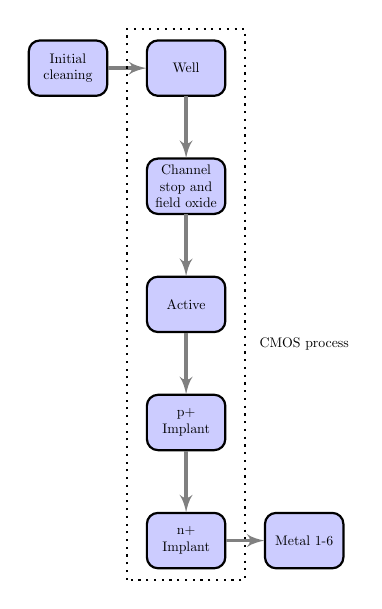
\begin{tikzpicture}[node distance = 3cm, auto, thick,scale=0.5, every node/.style={transform shape}]
				% Place nodes
				\node [block] (clean1) at (0,15) {Initial cleaning};
				\node [block, right of=clean1] (well) {Well};
				\node [block, below of=well] (fox) {Channel stop and field oxide};
				\node [block, below of=fox] (active) {Active};
				\node [block, below of=active] (pp) {p+ Implant};
				\node [block, below of=pp] (np) {n+ Implant};
				\node [block, right of=np] (metal) {Metal 1-6};
				% Draw edges
				\path [line] (clean1) -- (well);
				\path [line] (well) -- (fox);
				\path [line] (fox) -- (active);
				\path [line] (active) -- (pp);
				\path [line] (pp) -- (np);
				\path [line] (np) -- (metal);
				
				\draw[dotted] (1.5,2) rectangle (4.5,16);
				\node at (6,8) {CMOS process};
			\end{tikzpicture}
		\end{center}
		\caption{Frontend and backend process flow}
		\label{full_flow}
	\end{figure}
\end{center}

The five starting overall process steps are part of an overall active part of the technology, while the final metal (respectively contact) layers will be used for making a contact between the logic gates and macro cells and making them available to the exterior world.
For this process p-substrate is the required basic substrate, but forks and modifications will be very well possible based on a Graphene substrate or alike, still under the LSPL.
The decision to use an n-well approach is based largely on the compatibility with the existing nMOS process.
The starting material is a p-type, <100> oriented silicon with a doping concentration of $\approx 9\times10^{14}cm^{-3}$.

\newpage
\subsection{Initial cleaning}
In order to remove the initial naturally grown silicon dioxide from the wafer, acid is being applied to the wafer which leads to a pure silicon substrate wafer as in the process illustration shown below.

\begin{center}
	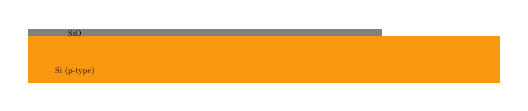
\begin{tikzpicture}[node distance = 3cm, auto, thick,scale=0.3, every node/.style={transform shape}]
		% substrate
		\fill[YellowOrange] (0,0) rectangle (20,2);
		\node at (2,0.5) {Si (p-type)};
		% oxide
		\fill[gray] (0,2) rectangle (15,2.3);
		\node at (2,2.1) {SiO};
	\end{tikzpicture}

	\includegraphics[scale=0.01]{down_arrow.png}

	
\begin{tikzpicture}[node distance = 3cm, auto, thick,scale=0.3, every node/.style={transform shape}]
		% substrate
		\fill[YellowOrange] (0,0) rectangle (20,2);
		\node at (2,0.5) {Si (p-type)};
	\end{tikzpicture}
\end{center}

This needs to be done because the naturally grown initially existing silicon oxide is not pure and may contain contamination which may render the final product unusable.

\subsubsection{Sulfuric Cleaning}
The sulfuric acid mixture, $H_2 S O_4 + H_2 O_2$ is being applied to the wafer for 10 minutes at a temperature of 120 \degree C.

\subsubsection{HF dip}
After the sulfuric cleaning a HF (HF:H$_2$O , 1:50) dip is being performed for one minute. \\
Hydrofluoric acid (HF) is used to remove native silicon dioxide from wafers. Since it acts quickly, one needs to only expose the wafer for a short time ("dip"). \\
After that the wafer needs to be dried and quickly processed further before new uncontrolled natural oxide can build up on the wafer through the contact with air.
\newpage
\subsection{Well}
In order to build CMOS (Complementary metal–oxide–semiconductor/P and N MOS) on the same substrate an n-well is required for building the complementary P-channel transistor for a n-p-channel logic circuitry as shown above in the example section.
The n-well will serve us as an island of n-doped substrate within the p-doped basis substrate.
The cross section as well as the top view of the targeted geometry are shown below.

\begin{center}
	\begin{tikzpicture}[node distance = 3cm, auto, thick,scale=0.3, every node/.style={transform shape}]
		\input{tikz_process_steps/2.a.tex}
	\end{tikzpicture}
	
\begin{tikzpicture}[node distance = 3cm, auto, thick,scale=0.3, every node/.style={transform shape}]
		% substrate
\fill[YellowOrange] (0,0) rectangle (20,12);
% n-well
\fill[Goldenrod] (1.25,1.5) rectangle (8.25,7.25);
	\end{tikzpicture}
\end{center}

\subsubsection{Dioxide layer}
In order to selectively inject charge carrying atoms into the crystalline structure a protective dioxide ($SiO_2$) layer needs to be grown on top of a p-type substrate.
\begin{center}
	\begin{tikzpicture}[node distance = 3cm, auto, thick,scale=0.3, every node/.style={transform shape}]
		\input{tikz_process_steps/2.1.a.tex}
	\end{tikzpicture} \\
	\includegraphics[scale=0.01]{down_arrow.png} \\
	\begin{tikzpicture}[node distance = 3cm, auto, thick,scale=0.3, every node/.style={transform shape}]
		\input{tikz_process_steps/2.1.b.tex}
	\end{tikzpicture}
\end{center}
The industrial best practice is a layer of around (500nm$\approx$5000\normalfont\AA) thickness or more.
For this purpose the wafer is being oxidized for at least 90 minutes at 1000\degree C using wet oxidation which results in a dioxide layer at least 500nm($\approx$5000\normalfont\AA) in thickness.

\subsubsection{Patterning}
The resist is being deposited using spin coating and then baked depending on the baking time for the specific resist.
The layout for being exposed onto the resist is being extracted from the "nwell" layer within the GDS2 file.
\begin{center}
	\begin{tikzpicture}[node distance = 3cm, auto, thick,scale=0.2, every node/.style={transform shape}]
		\input{tikz_process_steps/2.2.a.tex}
	\end{tikzpicture}
	\begin{tikzpicture}[node distance = 3cm, auto, thick,scale=0.2, every node/.style={transform shape}]
		\input{tikz_process_steps/2.2.at.tex}
	\end{tikzpicture} \\
	\includegraphics[scale=0.01]{down_arrow.png} \\
	\begin{tikzpicture}[node distance = 3cm, auto, thick,scale=0.2, every node/.style={transform shape}]
		\input{tikz_process_steps/2.2.b.tex}
	\end{tikzpicture}
	
\begin{tikzpicture}[node distance = 3cm, auto, thick,scale=0.2, every node/.style={transform shape}]
		% resist
\fill[orange] (0,0) rectangle (20,12);
% substrate
\fill[gray] (1.25,1.5) rectangle (8.25,7.25);
	\end{tikzpicture}
\end{center}
The thickness of the resist layer and the backing duration will variate depending on the specific equipment for which this process will be implemented with.

\subsubsection{Etching}
\begin{center}
	\begin{tikzpicture}[node distance = 3cm, auto, thick,scale=0.2, every node/.style={transform shape}]
		\input{tikz_process_steps/2.3.a.tex}
	\end{tikzpicture}
	\begin{tikzpicture}[node distance = 3cm, auto, thick,scale=0.2, every node/.style={transform shape}]
		\input{tikz_process_steps/2.3.at.tex}
	\end{tikzpicture} \\
	\includegraphics[scale=0.01]{down_arrow.png} \\
	\begin{tikzpicture}[node distance = 3cm, auto, thick,scale=0.2, every node/.style={transform shape}]
		\input{tikz_process_steps/2.3.b.tex}
	\end{tikzpicture}
	\begin{tikzpicture}[node distance = 3cm, auto, thick,scale=0.2, every node/.style={transform shape}]
		\input{tikz_process_steps/2.3.bt.tex}
	\end{tikzpicture}
\end{center}

\subsubsection{Cleaning}
\begin{center}
	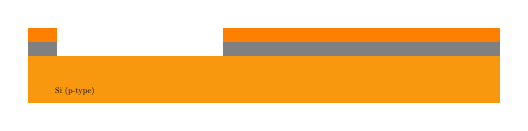
\begin{tikzpicture}[node distance = 3cm, auto, thick,scale=0.3, every node/.style={transform shape}]
		% substrate
		\fill[YellowOrange] (0,0) rectangle (20,2);
		\node at (2,0.5) {Si (p-type)};
		% oxide
		\fill[gray] (0,2) rectangle (1.25,2.6);
		\fill[gray] (8.25,2) rectangle (20,2.6);
		% resist
		\fill[orange] (0,2.6) rectangle (1.25,3.2);
		\fill[orange] (8.25,2.6) rectangle (20,3.2);
	\end{tikzpicture}

	\includegraphics[scale=0.01]{down_arrow.png}

	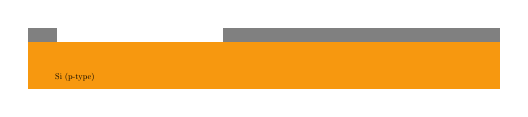
\begin{tikzpicture}[node distance = 3cm, auto, thick,scale=0.3, every node/.style={transform shape}]
		% substrate
		\fill[YellowOrange] (0,0) rectangle (20,2);
		\node at (2,0.5) {Si (p-type)};
		% oxide
		\fill[gray] (0,2) rectangle (1.25,2.6);
		\fill[gray] (8.25,2) rectangle (20,2.6);
	\end{tikzpicture}
\end{center}

\subsubsection{Predeposition}
\begin{center}
	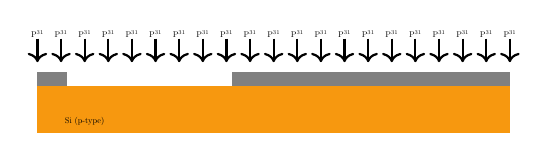
\begin{tikzpicture}[node distance = 3cm, auto, thick,scale=0.3, every node/.style={transform shape}]
		% substrate
		\fill[YellowOrange] (0,0) rectangle (20,2);
		\node at (2,0.5) {Si (p-type)};
		% oxide
		\fill[gray] (0,2) rectangle (1.25,2.6);
		\fill[gray] (8.25,2) rectangle (20,2.6);

		\newcounter{ct}
		\forloop{ct}{0}{\value{ct} < 21}
		{
			\draw [->] (\value{ct},4) -- (\value{ct},3);
			\node at (\value{ct},4.2) {P$^{31}$};
		}
	\end{tikzpicture}

	\includegraphics[scale=0.01]{down_arrow.png}

	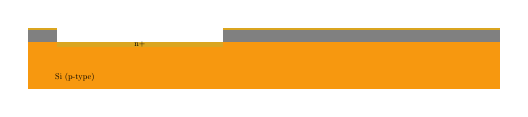
\begin{tikzpicture}[node distance = 3cm, auto, thick,scale=0.3, every node/.style={transform shape}]
		% substrate
		\fill[YellowOrange] (0,0) rectangle (20,2);
		\node at (2,0.5) {Si (p-type)};
		% phosphorus
		\fill[Goldenrod] (1.25,1.8) rectangle (8.25,2);
		\node at (4.75,1.9) {n+};
		% oxide
		\fill[gray] (0,2) rectangle (1.25,2.6);
		\fill[gray] (8.25,2) rectangle (20,2.6);

		\fill[Goldenrod] (0,2.5) rectangle (1.25,2.6);
		\fill[Goldenrod] (8.25,2.5) rectangle (20,2.6);
	\end{tikzpicture}
\end{center}

The n-well is implanted with a Phosphorus ($P^{31}$) dose of $2.5\times10^{12}cm^{-2}$ at an energy of 100 KeV.
The n-well is then annealed.

\subsubsection{Sacrificial oxide}
\begin{center}
	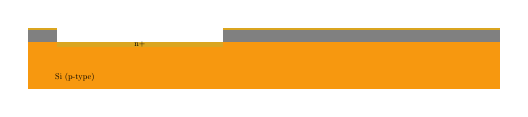
\begin{tikzpicture}[node distance = 3cm, auto, thick,scale=0.3, every node/.style={transform shape}]
		% substrate
		\fill[YellowOrange] (0,0) rectangle (20,2);
		\node at (2,0.5) {Si (p-type)};
		% phosphorus
		\fill[Goldenrod] (1.25,1.8) rectangle (8.25,2);
		\node at (4.75,1.9) {n+};
		% oxide
		\fill[gray] (0,2) rectangle (1.25,2.6);
		\fill[gray] (8.25,2) rectangle (20,2.6);

		\fill[Goldenrod] (0,2.5) rectangle (1.25,2.6);
		\fill[Goldenrod] (8.25,2.5) rectangle (20,2.6);
	\end{tikzpicture}

	\includegraphics[scale=0.01]{down_arrow.png}

	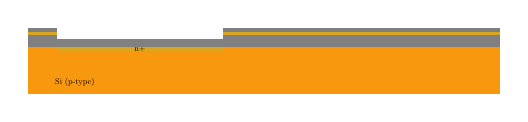
\begin{tikzpicture}[node distance = 3cm, auto, thick,scale=0.3, every node/.style={transform shape}]
		% substrate
		\fill[YellowOrange] (0,0) rectangle (20,2);
		\node at (2,0.5) {Si (p-type)};
		% phosphorus
		\fill[Goldenrod] (1.25,1.8) rectangle (8.25,2.0);
		\node at (4.75,1.9) {n+};
		% oxide
		\fill[gray] (0,2) rectangle (1.25,2.8);
		\fill[gray] (1.25,2) rectangle (8.25,2.3);
		\fill[gray] (8.25,2) rectangle (20,2.8);
		
		\fill[Goldenrod] (0,2.5) rectangle (1.25,2.6);
		\fill[Goldenrod] (8.25,2.5) rectangle (20,2.6);
	\end{tikzpicture}
\end{center}

The wafer is being oxidized for 32 minutes at 1000\degree C in order to achieve a cover silicon layer of 250nm thickness ($\approx$2500\normalfont\AA).

\subsubsection{Infusion}
In order to drive the carrier atoms deeper into the crystalline structure the wafer needs to be driven in after predeposition.
\begin{center}
	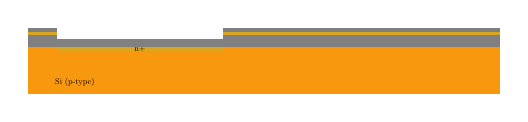
\begin{tikzpicture}[node distance = 3cm, auto, thick,scale=0.3, every node/.style={transform shape}]
		% substrate
		\fill[YellowOrange] (0,0) rectangle (20,2);
		\node at (2,0.5) {Si (p-type)};
		% phosphorus
		\fill[Goldenrod] (1.25,1.8) rectangle (8.25,2.0);
		\node at (4.75,1.9) {n+};
		% oxide
		\fill[gray] (0,2) rectangle (1.25,2.8);
		\fill[gray] (1.25,2) rectangle (8.25,2.3);
		\fill[gray] (8.25,2) rectangle (20,2.8);
		
		\fill[Goldenrod] (0,2.5) rectangle (1.25,2.6);
		\fill[Goldenrod] (8.25,2.5) rectangle (20,2.6);
	\end{tikzpicture}

	\includegraphics[scale=0.01]{down_arrow.png}

	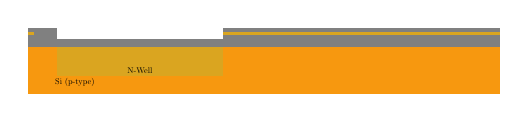
\begin{tikzpicture}[node distance = 3cm, auto, thick,scale=0.3, every node/.style={transform shape}]
		% substrate
		\fill[YellowOrange] (0,0) rectangle (20,2);
		\node at (2,0.5) {Si (p-type)};
		% n-well
		\fill[Goldenrod] (1.25,0.75) rectangle (8.25,2);
		\node at (4.75,1) {N-Well};
		% oxide
		\fill[gray] (0,2) rectangle (1.25,2.8);
		\fill[gray] (1.25,2) rectangle (8.25,2.3);
		\fill[gray] (8.25,2) rectangle (20,2.8);
		
		\fill[Goldenrod] (0,2.5) rectangle (0.25,2.6);
		\fill[Goldenrod] (8.25,2.5) rectangle (20,2.6);
	\end{tikzpicture}
\end{center}
In this step the wafer is  driven-in for 960 minutes at 1150\degree C in an inert ambient.

\subsubsection{Oxide removal}
We want an oxide free wafer with the n-well accessible for the further process steps.
\begin{center}
	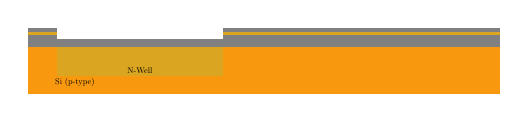
\begin{tikzpicture}[node distance = 3cm, auto, thick,scale=0.3, every node/.style={transform shape}]
		% substrate
		\fill[YellowOrange] (0,0) rectangle (20,2);
		\node at (2,0.5) {Si (p-type)};
		% n-well
		\fill[Goldenrod] (1.25,0.75) rectangle (8.25,2);
		\node at (4.75,1) {N-Well};
		% oxide
		\fill[gray] (0,2) rectangle (1.25,2.8);
		\fill[gray] (1.25,2) rectangle (8.25,2.3);
		\fill[gray] (8.25,2) rectangle (20,2.8);
		
		\fill[Goldenrod] (0,2.5) rectangle (1.25,2.6);
		\fill[Goldenrod] (8.25,2.5) rectangle (20,2.6);
	\end{tikzpicture}
	
	\includegraphics[scale=0.01]{down_arrow.png}

	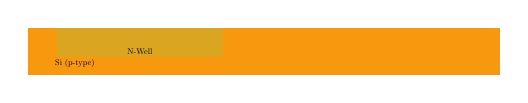
\begin{tikzpicture}[node distance = 3cm, auto, thick,scale=0.3, every node/.style={transform shape}]
		% substrate
		\fill[YellowOrange] (0,0) rectangle (20,2);
		\node at (2,0.5) {Si (p-type)};
		% n-well
		\fill[Goldenrod] (1.25,0.75) rectangle (8.25,2);
		\node at (4.75,1) {N-Well};
	\end{tikzpicture}
\end{center}

We use hydrofluoric acid, because it doesn't etch silicon at all but is very aggressive towards $SiO_2$

For hydrofluoric acid in combination with $SiO_2$ the following reaction formula can be used
\begin{equation}
4 H F_{(aq]} + SiO_{2(s]} \rightarrow SiF_{4(g]} \uparrow + 2 H_{2} O_{(l]}
\end{equation}
while with non oxidized silicon there is no reaction.
\newpage
\subsection{Channel stop and field oxide}

The channel-stop is material with the primary function to limit the spread of the channel area and to prevent the formation of parasitic channels.
It is a highly doped p+ area.
On top of the channel stop impurities is a thick layer of silicon oxide which has the primary function of isolating all the transistors from each other.

Its top view and cross section can be seen below.

\begin{center}
	\begin{tikzpicture}[node distance = 3cm, auto, thick,scale=0.3, every node/.style={transform shape}]
		\input{tikz_process_steps/3.a.tex}
	\end{tikzpicture}
	
\begin{tikzpicture}[node distance = 3cm, auto, thick,scale=0.3, every node/.style={transform shape}]
		% substrate
\fill[YellowOrange] (0,0) rectangle (20,12);
% n-well
\fill[Goldenrod] (1.25,1.5) rectangle (8.25,7.25);
% field oxide
\fill[DarkGray] (0,0) rectangle (1,12);
\fill[DarkGray] (8.5,0) rectangle (11.5,12);
\fill[DarkGray] (19,0) rectangle (20,12);
\fill[DarkGray] (0,0) rectangle (20,1.25);
\fill[DarkGray] (0,7.5) rectangle (20,12);
	\end{tikzpicture}
\end{center}

It surrounds all the active areas and covers all the non-active area.
The channel-stop region is always accompanied by the field oxide layer and shares the same layout mask with it.

\subsubsection{Dioxide layer}
\begin{center}
	\begin{tikzpicture}[node distance = 3cm, auto, thick,scale=0.3, every node/.style={transform shape}]
		\input{tikz_process_steps/3.1.a.tex}
	\end{tikzpicture} \\
	\includegraphics[scale=0.01]{down_arrow.png} \\
	\begin{tikzpicture}[node distance = 3cm, auto, thick,scale=0.3, every node/.style={transform shape}]
		\input{tikz_process_steps/3.1.b.tex}
	\end{tikzpicture}
\end{center}

\subsubsection{Nitride layer}
\begin{center}
	\begin{tikzpicture}[node distance = 3cm, auto, thick,scale=0.3, every node/.style={transform shape}]
		\input{tikz_process_steps/3.2.a.tex}
	\end{tikzpicture} \\
	\includegraphics[scale=0.01]{down_arrow.png} \\
	\begin{tikzpicture}[node distance = 3cm, auto, thick,scale=0.3, every node/.style={transform shape}]
		\input{tikz_process_steps/3.2.b.tex}
	\end{tikzpicture}
\end{center}

\subsubsection{Patterning}
\begin{center}
	\begin{tikzpicture}[node distance = 3cm, auto, thick,scale=0.2, every node/.style={transform shape}]
		\input{tikz_process_steps/3.3.a.tex}
	\end{tikzpicture}
	
\begin{tikzpicture}[node distance = 3cm, auto, thick,scale=0.2, every node/.style={transform shape}]
		\fill[purple] (0,0) rectangle (20,12);
	\end{tikzpicture} \\
	\includegraphics[scale=0.01]{down_arrow.png} \\
	\begin{tikzpicture}[node distance = 3cm, auto, thick,scale=0.2, every node/.style={transform shape}]
		\input{tikz_process_steps/3.3.b.tex}
	\end{tikzpicture}
	
\begin{tikzpicture}[node distance = 3cm, auto, thick,scale=0.2, every node/.style={transform shape}]
		\fill[purple] (0,0) rectangle (20,12);
\fill[orange] (1,1.25) rectangle (8.5,7.5);
\fill[orange] (11.5,1.25) rectangle (19,7.5);
	\end{tikzpicture}
\end{center}

\subsubsection{Etching}
\begin{center}
	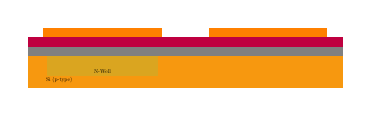
\begin{tikzpicture}[node distance = 3cm, auto, thick,scale=0.2, every node/.style={transform shape}]
		% substrate
\fill[YellowOrange] (0,0) rectangle (20,2);
\node at (2,0.5) {Si (p-type)};
% n-well
\fill[Goldenrod] (1.25,0.75) rectangle (8.25,2);
\node at (4.75,1) {N-Well};
% oxide
\fill[gray] (0,2) rectangle (20,2.6);
% nitride
\fill[purple] (0,2.6) rectangle (20,3.2);
% resist
\fill[orange] (1,3.2) rectangle (8.5,3.8);
\fill[orange] (11.5,3.2) rectangle (19,3.8);
	\end{tikzpicture}
	\begin{tikzpicture}[node distance = 3cm, auto, thick,scale=0.2, every node/.style={transform shape}]
		\input{tikz_process_steps/3.4.at.tex}
	\end{tikzpicture} \\
	\includegraphics[scale=0.01]{down_arrow.png} \\
	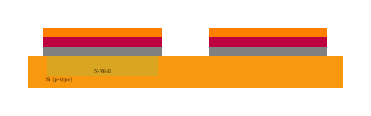
\begin{tikzpicture}[node distance = 3cm, auto, thick,scale=0.2, every node/.style={transform shape}]
		% substrate
\fill[YellowOrange] (0,0) rectangle (20,2);
\node at (2,0.5) {Si (p-type)};
% n-well
\fill[Goldenrod] (1.25,0.75) rectangle (8.25,2);
\node at (4.75,1) {N-Well};
% oxide
\fill[gray] (1,2) rectangle (8.5,2.6);
\fill[gray] (11.5,2) rectangle (19,2.6);
% nitride
\fill[purple] (1,2.6) rectangle (8.5,3.2);
\fill[purple] (11.5,2.6) rectangle (19,3.2);
% resist
\fill[orange] (1,3.2) rectangle (8.5,3.8);
\fill[orange] (11.5,3.2) rectangle (19,3.8);
	\end{tikzpicture}
	\begin{tikzpicture}[node distance = 3cm, auto, thick,scale=0.2, every node/.style={transform shape}]
		\input{tikz_process_steps/3.4.bt.tex}
	\end{tikzpicture}
\end{center}

\subsubsection{Cleaning}
\begin{center}
	\begin{tikzpicture}[node distance = 3cm, auto, thick,scale=0.3, every node/.style={transform shape}]
		\input{tikz_process_steps/3.5.a.tex}
	\end{tikzpicture} \\
	\includegraphics[scale=0.01]{down_arrow.png} \\
	\begin{tikzpicture}[node distance = 3cm, auto, thick,scale=0.3, every node/.style={transform shape}]
		\input{tikz_process_steps/3.5.b.tex}
	\end{tikzpicture}
\end{center}

\subsubsection{Injection}
\begin{center}
	\begin{tikzpicture}[node distance = 3cm, auto, thick,scale=0.3, every node/.style={transform shape}]
		% substrate
\fill[YellowOrange] (0,0) rectangle (20,2);
\node at (2,0.5) {Si (p-type)};
% n-well
\fill[Goldenrod] (1.25,0.75) rectangle (8.25,2);
\node at (4.75,1) {N-Well};
% oxide
\fill[gray] (1,2) rectangle (8.5,2.6);
\fill[gray] (11.5,2) rectangle (19,2.6);
% nitride
\fill[purple] (1,2.6) rectangle (8.5,3.2);
\fill[purple] (11.5,2.6) rectangle (19,3.2);

\forloop{ct}{0}{\value{ct} < 21}
{
	\draw [->] (\value{ct},4.5) -- (\value{ct},3.5);
	\node at (\value{ct},4.8) {B$^{11}$};
}
	\end{tikzpicture} \\
	\includegraphics[scale=0.01]{down_arrow.png} \\
	\begin{tikzpicture}[node distance = 3cm, auto, thick,scale=0.3, every node/.style={transform shape}]
		\input{tikz_process_steps/3.6.b.tex}
	\end{tikzpicture}
\end{center}

\subsubsection{Thick oxide layer}
The initial thickness of this field region is $\approx$7500\normalfont\AA, but is later reduced to $\approx$6000\normalfont\AA by various unmasked $SiO_2$ etches prior to  the polysilicon deposition.
\begin{center}
	\begin{tikzpicture}[node distance = 3cm, auto, thick,scale=0.3, every node/.style={transform shape}]
		\input{tikz_process_steps/3.7.a.tex}
	\end{tikzpicture} \\
	\includegraphics[scale=0.01]{down_arrow.png} \\
	\begin{tikzpicture}[node distance = 3cm, auto, thick,scale=0.3, every node/.style={transform shape}]
		\input{tikz_process_steps/3.7.b.tex}
	\end{tikzpicture}
\end{center}
The thick field oxide is grown in a pyrogenic steam ambient (partial pressure of $H_2O \approx  0.80\ atmospheres$) for 190 minutes at 1000 \degree C.

\subsubsection{Patterning}
\begin{center}
	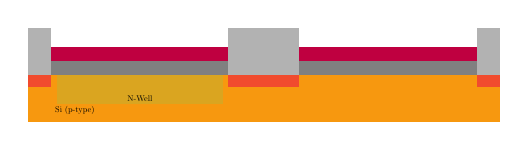
\begin{tikzpicture}[node distance = 3cm, auto, thick,scale=0.3, every node/.style={transform shape}]
		% substrate
\fill[YellowOrange] (0,0) rectangle (20,2);
\node at (2,0.5) {Si (p-type)};
% n-well
\fill[Goldenrod] (1.25,0.75) rectangle (8.25,2);
\node at (4.75,1) {N-Well};
% oxide
\fill[gray] (1,2) rectangle (8.5,2.6);
\fill[gray] (11.5,2) rectangle (19,2.6);
% nitride
\fill[purple] (1,2.6) rectangle (8.5,3.2);
\fill[purple] (11.5,2.6) rectangle (19,3.2);
% channel stop
\fill[RedOrange] (0,1.5) rectangle (1,2);
\fill[RedOrange] (8.5,1.5) rectangle (11.5,2);
\fill[RedOrange] (19,1.5) rectangle (20,2);
%field oxides:
\fill[DarkGray] (0,2) rectangle (1,4);
\fill[DarkGray] (8.5,2) rectangle (11.5,4);
\fill[DarkGray] (19,2) rectangle (20,4);
	\end{tikzpicture} \\
	\includegraphics[scale=0.01]{down_arrow.png} \\
	\begin{tikzpicture}[node distance = 3cm, auto, thick,scale=0.3, every node/.style={transform shape}]
		\input{tikz_process_steps/3.8.b.tex}
	\end{tikzpicture}
\end{center}

\subsubsection{Etching}
\begin{center}
	\begin{tikzpicture}[node distance = 3cm, auto, thick,scale=0.3, every node/.style={transform shape}]
		\input{tikz_process_steps/3.9.a.tex}
	\end{tikzpicture} \\
	\includegraphics[scale=0.01]{down_arrow.png} \\
	\begin{tikzpicture}[node distance = 3cm, auto, thick,scale=0.3, every node/.style={transform shape}]
		\input{tikz_process_steps/3.9.b.tex}
	\end{tikzpicture}
\end{center}
\newpage
\subsection{Active}
\begin{center}
	\begin{tikzpicture}[node distance = 3cm, auto, thick,scale=0.3, every node/.style={transform shape}]
		% substrate
		\fill[YellowOrange] (0,0) rectangle (20,2);
		\node at (2,0.5) {Si (p-type)};
		% n-well
		\fill[Goldenrod] (1.25,0.75) rectangle (8.25,2);
		\node at (4.75,1) {N-Well};
		% gate oxide
		\fill[LightGray] (4.8,2) rectangle (6.7,2.1);
		\fill[LightGray] (13.3,2) rectangle (15.2,2.1);
		% gate poly
		\fill[BrickRed] (4.8,2.1) rectangle (6.7,2.2);
		\fill[BrickRed] (13.3,2.1) rectangle (15.2,2.2);
		%field oxides:
		\fill[DarkGray] (0,2) rectangle (1,4);
		\fill[DarkGray] (8.5,2) rectangle (11.5,4);
		\fill[DarkGray] (19,2) rectangle (20,4);
		% channel stop
		\fill[RedOrange] (0,1.5) rectangle (1,2);
		\fill[RedOrange] (8.5,1.5) rectangle (11.5,2);
		\fill[RedOrange] (19,1.5) rectangle (20,2);
	\end{tikzpicture}
	\begin{tikzpicture}[node distance = 3cm, auto, thick,scale=0.3, every node/.style={transform shape}]
		\fill[YellowOrange] (0,0) rectangle (20,10);
		% n-well
		\fill[Goldenrod] (1.25,1.5) rectangle (8.25,7.25);
		% field oxide
		\fill[DarkGray] (0,0) rectangle (1,12);
		\fill[DarkGray] (8.5,0) rectangle (11.5,12);
		\fill[DarkGray] (19,0) rectangle (20,12);
		\fill[DarkGray] (0,0) rectangle (20,1.25);
		\fill[DarkGray] (0,7.5) rectangle (20,12);
		% poly
		\fill[BrickRed] (4.8,1.75) rectangle (6.7,9);
		\fill[BrickRed] (13.3,1.75) rectangle (15.2,9);
		\fill[BrickRed] (6.7,8) rectangle (15.2,9);
	\end{tikzpicture}
\end{center}

\subsubsection{Gate oxide growth}
The thickness of the gate oxide depends the capacity (slew rate) of the transistor.
The thinner the layer is, the steeper the edges of the CMOS circuitry will be, however also the threshold voltage will be reduced the thinner the gate oxide gets.

\begin{center}
	\begin{tikzpicture}[node distance = 3cm, auto, thick,scale=0.3, every node/.style={transform shape}]
		% substrate
		\fill[YellowOrange] (0,0) rectangle (20,2);
		\node at (2,0.5) {Si (p-type)};
		% n-well
		\fill[Goldenrod] (1.25,0.75) rectangle (8.25,2);
		\node at (4.75,1) {N-Well};
		%field oxides:
		\fill[DarkGray] (0,2) rectangle (1,4);
		\fill[DarkGray] (8.5,2) rectangle (11.5,4);
		\fill[DarkGray] (19,2) rectangle (20,4);
		% channel stop
		\fill[RedOrange] (0,1.5) rectangle (1,2);
		\fill[RedOrange] (8.5,1.5) rectangle (11.5,2);
		\fill[RedOrange] (19,1.5) rectangle (20,2);
	\end{tikzpicture}

	\includegraphics[scale=0.01]{down_arrow.png}
	
	\begin{tikzpicture}[node distance = 3cm, auto, thick,scale=0.3, every node/.style={transform shape}]
		% substrate
		\fill[YellowOrange] (0,0) rectangle (20,2);
		\node at (2,0.5) {Si (p-type)};
		% n-well
		\fill[Goldenrod] (1.25,0.75) rectangle (8.25,2);
		\node at (4.75,1) {N-Well};
		% gate oxide layer
		\fill[LightGray] (0,2) rectangle (20,2.1);
		%field oxides:
		\fill[DarkGray] (0,2) rectangle (1,4);
		\fill[DarkGray] (8.5,2) rectangle (11.5,4);
		\fill[DarkGray] (19,2) rectangle (20,4);
		% channel stop
		\fill[RedOrange] (0,1.5) rectangle (1,2);
		\fill[RedOrange] (8.5,1.5) rectangle (11.5,2);
		\fill[RedOrange] (19,1.5) rectangle (20,2);
	\end{tikzpicture}
\end{center}

\subsubsection{Polysilicon growth}
\begin{center}
	\begin{tikzpicture}[node distance = 3cm, auto, thick,scale=0.3, every node/.style={transform shape}]
		% substrate
		\fill[YellowOrange] (0,0) rectangle (20,2);
		\node at (2,0.5) {Si (p-type)};
		% n-well
		\fill[Goldenrod] (1.25,0.75) rectangle (8.25,2);
		\node at (4.75,1) {N-Well};
		% gate oxide layer
		\fill[LightGray] (0,2) rectangle (20,2.1);
		%field oxides:
		\fill[DarkGray] (0,2) rectangle (1,4);
		\fill[DarkGray] (8.5,2) rectangle (11.5,4);
		\fill[DarkGray] (19,2) rectangle (20,4);
		% channel stop
		\fill[RedOrange] (0,1.5) rectangle (1,2);
		\fill[RedOrange] (8.5,1.5) rectangle (11.5,2);
		\fill[RedOrange] (19,1.5) rectangle (20,2);
	\end{tikzpicture}

	\includegraphics[scale=0.01]{down_arrow.png}

	\begin{tikzpicture}[node distance = 3cm, auto, thick,scale=0.3, every node/.style={transform shape}]
		% substrate
		\fill[YellowOrange] (0,0) rectangle (20,2);
		\node at (2,0.5) {Si (p-type)};
		% n-well
		\fill[Goldenrod] (1.25,0.75) rectangle (8.25,2);
		\node at (4.75,1) {N-Well};
		% gate oxide layer
		\fill[LightGray] (0,2) rectangle (20,2.1);
		% poly layer
		\fill[BrickRed] (0,2.1) rectangle (20,2.2);
		%field oxides:
		\fill[DarkGray] (0,2) rectangle (1,4);
		\fill[DarkGray] (8.5,2) rectangle (11.5,4);
		\fill[DarkGray] (19,2) rectangle (20,4);
		% channel stop
		\fill[RedOrange] (0,1.5) rectangle (1,2);
		\fill[RedOrange] (8.5,1.5) rectangle (11.5,2);
		\fill[RedOrange] (19,1.5) rectangle (20,2);
	\end{tikzpicture}
\end{center}

\subsubsection{Patterning}
\begin{center}
	\begin{tikzpicture}[node distance = 3cm, auto, thick,scale=0.2, every node/.style={transform shape}]
		% substrate
		\fill[YellowOrange] (0,0) rectangle (20,2);
		\node at (2,0.5) {Si (p-type)};
		% n-well
		\fill[Goldenrod] (1.25,0.75) rectangle (8.25,2);
		\node at (4.75,1) {N-Well};
		% gate oxide layer
		\fill[LightGray] (0,2) rectangle (20,2.1);
		% poly layer
		\fill[BrickRed] (0,2.1) rectangle (20,2.2);
		%field oxides:
		\fill[DarkGray] (0,2) rectangle (1,4);
		\fill[DarkGray] (8.5,2) rectangle (11.5,4);
		\fill[DarkGray] (19,2) rectangle (20,4);
		% channel stop
		\fill[RedOrange] (0,1.5) rectangle (1,2);
		\fill[RedOrange] (8.5,1.5) rectangle (11.5,2);
		\fill[RedOrange] (19,1.5) rectangle (20,2);
	\end{tikzpicture}
	\begin{tikzpicture}[node distance = 3cm, auto, thick,scale=0.2, every node/.style={transform shape}]
		\fill[BrickRed] (0,0) rectangle (20,10);
	\end{tikzpicture}

	\includegraphics[scale=0.01]{down_arrow.png}

	\begin{tikzpicture}[node distance = 3cm, auto, thick,scale=0.2, every node/.style={transform shape}]
		% substrate
		\fill[YellowOrange] (0,0) rectangle (20,2);
		\node at (2,0.5) {Si (p-type)};
		% n-well
		\fill[Goldenrod] (1.25,0.75) rectangle (8.25,2);
		\node at (4.75,1) {N-Well};
		% gate oxide layer
		\fill[LightGray] (0,2) rectangle (20,2.1);
		% poly layer
		\fill[BrickRed] (0,2.1) rectangle (20,2.2);
		% resist
		\fill[orange] (4.8,2.2) rectangle (6.7,2.8);
		\fill[orange] (13.3,2.2) rectangle (15.2,2.8);
		%field oxides:
		\fill[DarkGray] (0,2) rectangle (1,4);
		\fill[DarkGray] (8.5,2) rectangle (11.5,4);
		\fill[DarkGray] (19,2) rectangle (20,4);
		% channel stop
		\fill[RedOrange] (0,1.5) rectangle (1,2);
		\fill[RedOrange] (8.5,1.5) rectangle (11.5,2);
		\fill[RedOrange] (19,1.5) rectangle (20,2);
	\end{tikzpicture}
	\begin{tikzpicture}[node distance = 3cm, auto, thick,scale=0.2, every node/.style={transform shape}]
		\fill[BrickRed] (0,0) rectangle (20,10);
		% resist
		\fill[orange] (4.8,1.75) rectangle (6.7,9);
		\fill[orange] (13.3,1.75) rectangle (15.2,9);
		\fill[orange] (6.7,8) rectangle (15.2,9);
	\end{tikzpicture}
\end{center}

\subsubsection{Etching}
\begin{center}
	\begin{tikzpicture}[node distance = 3cm, auto, thick,scale=0.2, every node/.style={transform shape}]
		% substrate
		\fill[YellowOrange] (0,0) rectangle (20,2);
		\node at (2,0.5) {Si (p-type)};
		% n-well
		\fill[Goldenrod] (1.25,0.75) rectangle (8.25,2);
		\node at (4.75,1) {N-Well};
		% gate oxide layer
		\fill[LightGray] (0,2) rectangle (20,2.1);
		% poly layer
		\fill[BrickRed] (0,2.1) rectangle (20,2.2);
		% resist
		\fill[orange] (4.8,2.2) rectangle (6.7,2.8);
		\fill[orange] (13.3,2.2) rectangle (15.2,2.8);
		%field oxides:
		\fill[DarkGray] (0,2) rectangle (1,4);
		\fill[DarkGray] (8.5,2) rectangle (11.5,4);
		\fill[DarkGray] (19,2) rectangle (20,4);
		% channel stop
		\fill[RedOrange] (0,1.5) rectangle (1,2);
		\fill[RedOrange] (8.5,1.5) rectangle (11.5,2);
		\fill[RedOrange] (19,1.5) rectangle (20,2);
	\end{tikzpicture}
	\begin{tikzpicture}[node distance = 3cm, auto, thick,scale=0.2, every node/.style={transform shape}]
		\fill[BrickRed] (0,0) rectangle (20,10);
		% resist
		\fill[orange] (4.8,1.75) rectangle (6.7,9);
		\fill[orange] (13.3,1.75) rectangle (15.2,9);
		\fill[orange] (4.8,8) rectangle (15.2,9);
	\end{tikzpicture}

	\includegraphics[scale=0.01]{down_arrow.png}

	\begin{tikzpicture}[node distance = 3cm, auto, thick,scale=0.2, every node/.style={transform shape}]
		% substrate
		\fill[YellowOrange] (0,0) rectangle (20,2);
		\node at (2,0.5) {Si (p-type)};
		% n-well
		\fill[Goldenrod] (1.25,0.75) rectangle (8.25,2);
		\node at (4.75,1) {N-Well};
		% gate oxide
		\fill[LightGray] (4.8,2) rectangle (6.7,2.1);
		\fill[LightGray] (13.3,2) rectangle (15.2,2.1);
		% gate poly
		\fill[BrickRed] (4.8,2.1) rectangle (6.7,2.2);
		\fill[BrickRed] (13.3,2.1) rectangle (15.2,2.2);
		% resist
		\fill[orange] (4.8,2.2) rectangle (6.7,2.8);
		\fill[orange] (13.3,2.2) rectangle (15.2,2.8);
		%field oxides:
		\fill[DarkGray] (0,2) rectangle (1,4);
		\fill[DarkGray] (8.5,2) rectangle (11.5,4);
		\fill[DarkGray] (19,2) rectangle (20,4);
		% channel stop
		\fill[RedOrange] (0,1.5) rectangle (1,2);
		\fill[RedOrange] (8.5,1.5) rectangle (11.5,2);
		\fill[RedOrange] (19,1.5) rectangle (20,2);
	\end{tikzpicture}
	\begin{tikzpicture}[node distance = 3cm, auto, thick,scale=0.2, every node/.style={transform shape}]
		\fill[YellowOrange] (0,0) rectangle (20,10);
		% n-well
		\fill[Goldenrod] (1.25,1.5) rectangle (8.25,7.25);
		% field oxide
		\fill[DarkGray] (0,0) rectangle (1,12);
		\fill[DarkGray] (8.5,0) rectangle (11.5,12);
		\fill[DarkGray] (19,0) rectangle (20,12);
		\fill[DarkGray] (0,0) rectangle (20,1.25);
		\fill[DarkGray] (0,7.5) rectangle (20,12);
		% resist
		\fill[orange] (4.8,1.75) rectangle (6.7,9);
		\fill[orange] (13.3,1.75) rectangle (15.2,9);
		\fill[orange] (4.8,8) rectangle (15.2,9);
	\end{tikzpicture}
\end{center}
Because the exact shape of the gate contact is required for a reproducible property characterization of the transistor geometry, dry etching is being used for etching the poly-oxide layer stack.

\subsubsection{Cleaning}
\begin{center}
	\begin{tikzpicture}[node distance = 3cm, auto, thick,scale=0.2, every node/.style={transform shape}]
		% substrate
		\fill[YellowOrange] (0,0) rectangle (20,2);
		\node at (2,0.5) {Si (p-type)};
		% n-well
		\fill[Goldenrod] (1.25,0.75) rectangle (8.25,2);
		\node at (4.75,1) {N-Well};
		% gate oxide
		\fill[LightGray] (4.8,2) rectangle (6.7,2.1);
		\fill[LightGray] (13.3,2) rectangle (15.2,2.1);
		% gate poly
		\fill[BrickRed] (4.8,2.1) rectangle (6.7,2.2);
		\fill[BrickRed] (13.3,2.1) rectangle (15.2,2.2);
		% resist
		\fill[orange] (4.8,2.2) rectangle (6.7,2.8);
		\fill[orange] (13.3,2.2) rectangle (15.2,2.8);
		%field oxides:
		\fill[DarkGray] (0,2) rectangle (1,4);
		\fill[DarkGray] (8.5,2) rectangle (11.5,4);
		\fill[DarkGray] (19,2) rectangle (20,4);
		% channel stop
		\fill[RedOrange] (0,1.5) rectangle (1,2);
		\fill[RedOrange] (8.5,1.5) rectangle (11.5,2);
		\fill[RedOrange] (19,1.5) rectangle (20,2);
	\end{tikzpicture}
	\begin{tikzpicture}[node distance = 3cm, auto, thick,scale=0.2, every node/.style={transform shape}]
		\fill[YellowOrange] (0,0) rectangle (20,10);
		% n-well
		\fill[Goldenrod] (1.25,1.5) rectangle (8.25,7.25);
		% field oxide
		\fill[DarkGray] (0,0) rectangle (1,12);
		\fill[DarkGray] (8.5,0) rectangle (11.5,12);
		\fill[DarkGray] (19,0) rectangle (20,12);
		\fill[DarkGray] (0,0) rectangle (20,1.25);
		\fill[DarkGray] (0,7.5) rectangle (20,12);
		% resist
		\fill[orange] (4.8,1.75) rectangle (6.7,9);
		\fill[orange] (13.3,1.75) rectangle (15.2,9);
		\fill[orange] (4.8,8) rectangle (15.2,9);
	\end{tikzpicture}

	\includegraphics[scale=0.01]{down_arrow.png}

	\begin{tikzpicture}[node distance = 3cm, auto, thick,scale=0.2, every node/.style={transform shape}]
		% substrate
		\fill[YellowOrange] (0,0) rectangle (20,2);
		\node at (2,0.5) {Si (p-type)};
		% n-well
		\fill[Goldenrod] (1.25,0.75) rectangle (8.25,2);
		\node at (4.75,1) {N-Well};
		% gate oxide
		\fill[LightGray] (4.8,2) rectangle (6.7,2.1);
		\fill[LightGray] (13.3,2) rectangle (15.2,2.1);
		% gate poly
		\fill[BrickRed] (4.8,2.1) rectangle (6.7,2.2);
		\fill[BrickRed] (13.3,2.1) rectangle (15.2,2.2);
		%field oxides:
		\fill[DarkGray] (0,2) rectangle (1,4);
		\fill[DarkGray] (8.5,2) rectangle (11.5,4);
		\fill[DarkGray] (19,2) rectangle (20,4);
		% channel stop
		\fill[RedOrange] (0,1.5) rectangle (1,2);
		\fill[RedOrange] (8.5,1.5) rectangle (11.5,2);
		\fill[RedOrange] (19,1.5) rectangle (20,2);
	\end{tikzpicture}
	\begin{tikzpicture}[node distance = 3cm, auto, thick,scale=0.2, every node/.style={transform shape}]
		\fill[YellowOrange] (0,0) rectangle (20,10);
		% n-well
		\fill[Goldenrod] (1.25,1.5) rectangle (8.25,7.25);
		% field oxide
		\fill[DarkGray] (0,0) rectangle (1,12);
		\fill[DarkGray] (8.5,0) rectangle (11.5,12);
		\fill[DarkGray] (19,0) rectangle (20,12);
		\fill[DarkGray] (0,0) rectangle (20,1.25);
		\fill[DarkGray] (0,7.5) rectangle (20,12);
		% poly
		\fill[BrickRed] (4.8,1.75) rectangle (6.7,9);
		\fill[BrickRed] (13.3,1.75) rectangle (15.2,9);
		\fill[BrickRed] (4.8,8) rectangle (15.2,9);
	\end{tikzpicture}
\end{center}

\newpage

\subsection{p+ Implant}
\begin{center}
	\begin{tikzpicture}[node distance = 3cm, auto, thick,scale=0.3, every node/.style={transform shape}]
		% substrate
		\fill[YellowOrange] (0,0) rectangle (20,2);
		% n-well
		\fill[Goldenrod] (1.25,0.75) rectangle (8.25,2);
		% source
		\fill[RedOrange] (0,1.5) rectangle (1,2);
		\fill[RedOrange] (3.5,1) rectangle (5,2);
		\fill[RedOrange] (6.5,1) rectangle (8,2);
		\fill[RedOrange] (8.5,1.5) rectangle (11.5,2);
		\fill[RedOrange] (17,1) rectangle (18.5,2);
		\fill[RedOrange] (19,1.5) rectangle (20,2);
		% gate oxide
		\fill[LightGray] (4.8,2) rectangle (6.7,2.1);
		\fill[LightGray] (13.3,2) rectangle (15.2,2.1);
		% gate poly
		\fill[BrickRed] (4.8,2.1) rectangle (6.7,2.2);
		\fill[BrickRed] (13.3,2.1) rectangle (15.2,2.2);
		%field oxides:
		\fill[DarkGray] (0,2) rectangle (1,4);
		\fill[DarkGray] (8.5,2) rectangle (11.5,4);
		\fill[DarkGray] (19,2) rectangle (20,4);
		% channel stop
		\fill[RedOrange] (0,1.5) rectangle (1,2);
		\fill[RedOrange] (8.5,1.5) rectangle (11.5,2);
		\fill[RedOrange] (19,1.5) rectangle (20,2);
	\end{tikzpicture}
	\begin{tikzpicture}[node distance = 3cm, auto, thick,scale=0.3, every node/.style={transform shape}]
		\fill[YellowOrange] (0,0) rectangle (20,10);
		% n-well
		\fill[Goldenrod] (1.25,1.5) rectangle (8.25,7.25);
		% p+
		\fill[RedOrange] (3.5,2) rectangle (5,6.5);
		\fill[RedOrange] (6.5,2) rectangle (8,6.5);
		\fill[RedOrange] (17,2) rectangle (18.5,6.5);
		% field oxide
		\fill[DarkGray] (0,0) rectangle (1,12);
		\fill[DarkGray] (8.5,0) rectangle (11.5,12);
		\fill[DarkGray] (19,0) rectangle (20,12);
		\fill[DarkGray] (0,0) rectangle (20,1.25);
		\fill[DarkGray] (0,7.5) rectangle (20,12);
		% poly
		\fill[BrickRed] (4.8,1.75) rectangle (6.7,9);
		\fill[BrickRed] (13.3,1.75) rectangle (15.2,9);
		\fill[BrickRed] (4.8,8) rectangle (15.2,9);
	\end{tikzpicture}
\end{center}

For the bulk of the NMOS transistors and for the source and drain of the PMOS transistors highly doped  p+ areas are required.
In this step we're going to build these.

\subsubsection{Dioxide layer}
\begin{center}
	\begin{tikzpicture}[node distance = 3cm, auto, thick,scale=0.4, every node/.style={transform shape}]
		% substrate
		\fill[YellowOrange] (0,0) rectangle (20,2);
		\node at (2,0.5) {Si (p-type)};
		% n-well
		\fill[Goldenrod] (1.25,0.75) rectangle (8.25,2);
		\node at (4.75,1) {N-Well};
		% gate oxide
		\fill[LightGray] (4.8,2) rectangle (6.7,2.1);
		\fill[LightGray] (13.3,2) rectangle (15.2,2.1);
		% gate poly
		\fill[BrickRed] (4.8,2.1) rectangle (6.7,2.2);
		\fill[BrickRed] (13.3,2.1) rectangle (15.2,2.2);
		%field oxides:
		\fill[DarkGray] (0,2) rectangle (1,4);
		\fill[DarkGray] (8.5,2) rectangle (11.5,4);
		\fill[DarkGray] (19,2) rectangle (20,4);
		% channel stop
		\fill[RedOrange] (0,1.5) rectangle (1,2);
		\fill[RedOrange] (8.5,1.5) rectangle (11.5,2);
		\fill[RedOrange] (19,1.5) rectangle (20,2);
	\end{tikzpicture}

	\includegraphics[scale=0.01]{down_arrow.png}
	
	\begin{tikzpicture}[node distance = 3cm, auto, thick,scale=0.4, every node/.style={transform shape}]
		% substrate
		\fill[YellowOrange] (0,0) rectangle (20,2);
		\node at (2,0.5) {Si (p-type)};
		% n-well
		\fill[Goldenrod] (1.25,0.75) rectangle (8.25,2);
		\node at (4.75,1) {N-Well};
		% gate oxide
		\fill[LightGray] (4.8,2) rectangle (6.7,2.1);
		\fill[LightGray] (13.3,2) rectangle (15.2,2.1);
		% gate poly
		\fill[BrickRed] (4.8,2.1) rectangle (6.7,2.2);
		\fill[BrickRed] (13.3,2.1) rectangle (15.2,2.2);
		% dioxide
		\fill[NormalGray] (0,2) rectangle (4.8,2.7);
		\fill[NormalGray] (4.8,2.2) rectangle (6.7,2.7);
		\fill[NormalGray] (6.7,2) rectangle (13.3,2.7);
		\fill[NormalGray] (13.3,2.2) rectangle (15.2,2.7);
		\fill[NormalGray] (15.2,2) rectangle (20,2.7);
		%field oxides:
		\fill[DarkGray] (0,2) rectangle (1,4);
		\fill[DarkGray] (8.5,2) rectangle (11.5,4);
		\fill[DarkGray] (19,2) rectangle (20,4);
		% channel stop
		\fill[RedOrange] (0,1.5) rectangle (1,2);
		\fill[RedOrange] (8.5,1.5) rectangle (11.5,2);
		\fill[RedOrange] (19,1.5) rectangle (20,2);
	\end{tikzpicture}
\end{center}

\subsubsection{Pattering}
\begin{center}
	\begin{tikzpicture}[node distance = 3cm, auto, thick,scale=0.2, every node/.style={transform shape}]
		% substrate
		\fill[YellowOrange] (0,0) rectangle (20,2);
		\node at (2,0.5) {Si (p-type)};
		% n-well
		\fill[Goldenrod] (1.25,0.75) rectangle (8.25,2);
		\node at (4.75,1) {N-Well};
		% gate oxide
		\fill[LightGray] (4.8,2) rectangle (6.7,2.1);
		\fill[LightGray] (13.3,2) rectangle (15.2,2.1);
		% gate poly
		\fill[BrickRed] (4.8,2.1) rectangle (6.7,2.2);
		\fill[BrickRed] (13.3,2.1) rectangle (15.2,2.2);
		% dioxide
		\fill[NormalGray] (0,2) rectangle (4.8,2.7);
		\fill[NormalGray] (4.8,2.2) rectangle (6.7,2.7);
		\fill[NormalGray] (6.7,2) rectangle (13.3,2.7);
		\fill[NormalGray] (13.3,2.2) rectangle (15.2,2.7);
		\fill[NormalGray] (15.2,2) rectangle (20,2.7);
		%field oxides:
		\fill[DarkGray] (0,2) rectangle (1,4);
		\fill[DarkGray] (8.5,2) rectangle (11.5,4);
		\fill[DarkGray] (19,2) rectangle (20,4);
		% channel stop
		\fill[RedOrange] (0,1.5) rectangle (1,2);
		\fill[RedOrange] (8.5,1.5) rectangle (11.5,2);
		\fill[RedOrange] (19,1.5) rectangle (20,2);
	\end{tikzpicture}
	\begin{tikzpicture}[node distance = 3cm, auto, thick,scale=0.2, every node/.style={transform shape}]
		\fill[NormalGray] (0,0) rectangle (20,12);
	\end{tikzpicture}

	\includegraphics[scale=0.01]{down_arrow.png}

	\begin{tikzpicture}[node distance = 3cm, auto, thick,scale=0.2, every node/.style={transform shape}]
		% substrate
		\fill[YellowOrange] (0,0) rectangle (20,2);
		\node at (2,0.5) {Si (p-type)};
		% n-well
		\fill[Goldenrod] (1.25,0.75) rectangle (8.25,2);
		\node at (4.75,1) {N-Well};
		% gate oxide
		\fill[LightGray] (4.8,2) rectangle (6.7,2.1);
		\fill[LightGray] (13.3,2) rectangle (15.2,2.1);
		% gate poly
		\fill[BrickRed] (4.8,2.1) rectangle (6.7,2.2);
		\fill[BrickRed] (13.3,2.1) rectangle (15.2,2.2);
		% dioxide
		\fill[NormalGray] (0,2) rectangle (4.8,2.7);
		\fill[NormalGray] (4.8,2.2) rectangle (6.7,2.7);
		\fill[NormalGray] (6.7,2) rectangle (13.3,2.7);
		\fill[NormalGray] (13.3,2.2) rectangle (15.2,2.7);
		\fill[NormalGray] (15.2,2) rectangle (20,2.7);
		% resist
		\fill[orange] (0,4) rectangle (1,4.6);
		\fill[orange] (1,2.7) rectangle (3.5,4.6);
		\fill[orange] (8,2.7) rectangle (8.5,4.6);
		\fill[orange] (8.5,4) rectangle (11.5,4.6);
		\fill[orange] (11.5,2.7) rectangle (17,4.6);
		\fill[orange] (18.5,2.7) rectangle (19,4.6);
		\fill[orange] (19,4) rectangle (20,4.6);
		%field oxides:
		\fill[DarkGray] (0,2) rectangle (1,4);
		\fill[DarkGray] (8.5,2) rectangle (11.5,4);
		\fill[DarkGray] (19,2) rectangle (20,4);
		% channel stop
		\fill[RedOrange] (0,1.5) rectangle (1,2);
		\fill[RedOrange] (8.5,1.5) rectangle (11.5,2);
		\fill[RedOrange] (19,1.5) rectangle (20,2);
	\end{tikzpicture}
	\begin{tikzpicture}[node distance = 3cm, auto, thick,scale=0.2, every node/.style={transform shape}]
		\fill[orange] (0,0) rectangle (20,12);
		\fill[NormalGray] (3.5,2) rectangle (8,6.5);
		\fill[NormalGray] (17,2) rectangle (18.5,6.5);
	\end{tikzpicture}
\end{center}

\subsubsection{Etching}
\begin{center}
	\begin{tikzpicture}[node distance = 3cm, auto, thick,scale=0.2, every node/.style={transform shape}]
		% substrate
		\fill[YellowOrange] (0,0) rectangle (20,2);
		\node at (2,0.5) {Si (p-type)};
		% n-well
		\fill[Goldenrod] (1.25,0.75) rectangle (8.25,2);
		\node at (4.75,1) {N-Well};
		% gate oxide
		\fill[LightGray] (4.8,2) rectangle (6.7,2.1);
		\fill[LightGray] (13.3,2) rectangle (15.2,2.1);
		% gate poly
		\fill[BrickRed] (4.8,2.1) rectangle (6.7,2.2);
		\fill[BrickRed] (13.3,2.1) rectangle (15.2,2.2);
		% dioxide
		\fill[NormalGray] (0,2) rectangle (4.8,2.7);
		\fill[NormalGray] (4.8,2.2) rectangle (6.7,2.7);
		\fill[NormalGray] (6.7,2) rectangle (13.3,2.7);
		\fill[NormalGray] (13.3,2.2) rectangle (15.2,2.7);
		\fill[NormalGray] (15.2,2) rectangle (20,2.7);
		% resist
		\fill[orange] (0,4) rectangle (1,4.6);
		\fill[orange] (1,2.7) rectangle (3.5,4.6);
		\fill[orange] (8,2.7) rectangle (8.5,4.6);
		\fill[orange] (8.5,4) rectangle (11.5,4.6);
		\fill[orange] (11.5,2.7) rectangle (17,4.6);
		\fill[orange] (18.5,2.7) rectangle (19,4.6);
		\fill[orange] (19,4) rectangle (20,4.6);
		%field oxides:
		\fill[DarkGray] (0,2) rectangle (1,4);
		\fill[DarkGray] (8.5,2) rectangle (11.5,4);
		\fill[DarkGray] (19,2) rectangle (20,4);
		% channel stop
		\fill[RedOrange] (0,1.5) rectangle (1,2);
		\fill[RedOrange] (8.5,1.5) rectangle (11.5,2);
		\fill[RedOrange] (19,1.5) rectangle (20,2);
	\end{tikzpicture}
	\begin{tikzpicture}[node distance = 3cm, auto, thick,scale=0.2, every node/.style={transform shape}]
		\fill[orange] (0,0) rectangle (20,12);
		\fill[NormalGray] (3.5,2) rectangle (8,6.5);
		\fill[NormalGray] (17,2) rectangle (18.5,6.5);
	\end{tikzpicture}

	\includegraphics[scale=0.01]{down_arrow.png}

	\begin{tikzpicture}[node distance = 3cm, auto, thick,scale=0.2, every node/.style={transform shape}]
		% substrate
		\fill[YellowOrange] (0,0) rectangle (20,2);
		\node at (2,0.5) {Si (p-type)};
		% n-well
		\fill[Goldenrod] (1.25,0.75) rectangle (8.25,2);
		\node at (4.75,1) {N-Well};
		% gate oxide
		\fill[LightGray] (4.8,2) rectangle (6.7,2.1);
		\fill[LightGray] (13.3,2) rectangle (15.2,2.1);
		% gate poly
		\fill[BrickRed] (4.8,2.1) rectangle (6.7,2.2);
		\fill[BrickRed] (13.3,2.1) rectangle (15.2,2.2);
		% dioxide
		\fill[NormalGray] (0,2) rectangle (3.5,2.7);
		\fill[NormalGray] (8,2) rectangle (13.3,2.7);
		\fill[NormalGray] (13.3,2.2) rectangle (15.2,2.7);
		\fill[NormalGray] (15.2,2) rectangle (17,2.7);
		\fill[NormalGray] (18.5,2) rectangle (20,2.7);
		% resist
		\fill[orange] (0,4) rectangle (1,4.6);
		\fill[orange] (1,2.7) rectangle (3.5,3.3);
		\fill[orange] (8,2.7) rectangle (8.5,3.3);
		\fill[orange] (8.5,4) rectangle (11.5,4.6);
		\fill[orange] (11.5,2.7) rectangle (17,3.3);
		\fill[orange] (18.5,2.7) rectangle (19,3.3);
		\fill[orange] (19,4) rectangle (20,4.6);
		%field oxides:
		\fill[DarkGray] (0,2) rectangle (1,4);
		\fill[DarkGray] (8.5,2) rectangle (11.5,4);
		\fill[DarkGray] (19,2) rectangle (20,4);
		% channel stop
		\fill[RedOrange] (0,1.5) rectangle (1,2);
		\fill[RedOrange] (8.5,1.5) rectangle (11.5,2);
		\fill[RedOrange] (19,1.5) rectangle (20,2);
	\end{tikzpicture}
	\begin{tikzpicture}[node distance = 3cm, auto, thick,scale=0.2, every node/.style={transform shape}]
		\fill[orange] (0,0) rectangle (20,12);
		% source & drain
		\fill[Goldenrod] (2.5,1.5) rectangle (7,6);
		% body
		\fill[YellowOrange] (17,1.5) rectangle (18.5,6);
		% gate poly
		\fill[BrickRed] (3.8,1.5) rectangle (5.7,6);
	\end{tikzpicture}
\end{center}

\subsubsection{Cleaning}
\begin{center}
	\begin{tikzpicture}[node distance = 3cm, auto, thick,scale=0.3, every node/.style={transform shape}]
		% substrate
		\fill[YellowOrange] (0,0) rectangle (20,2);
		\node at (2,0.5) {Si (p-type)};
		% n-well
		\fill[Goldenrod] (1.25,0.75) rectangle (8.25,2);
		\node at (4.75,1) {N-Well};
		% gate oxide
		\fill[LightGray] (4.8,2) rectangle (6.7,2.1);
		\fill[LightGray] (13.3,2) rectangle (15.2,2.1);
		% gate poly
		\fill[BrickRed] (4.8,2.1) rectangle (6.7,2.2);
		\fill[BrickRed] (13.3,2.1) rectangle (15.2,2.2);
		% dioxide
		\fill[NormalGray] (0,2) rectangle (3.5,2.7);
		\fill[NormalGray] (8,2) rectangle (13.3,2.7);
		\fill[NormalGray] (13.3,2.2) rectangle (15.2,2.7);
		\fill[NormalGray] (15.2,2) rectangle (17,2.7);
		\fill[NormalGray] (18.5,2) rectangle (20,2.7);
		% resist
		\fill[orange] (0,4) rectangle (1,4.6);
		\fill[orange] (1,2.7) rectangle (3.5,4.6);
		\fill[orange] (8,2.7) rectangle (8.5,4.6);
		\fill[orange] (8.5,4) rectangle (11.5,4.6);
		\fill[orange] (11.5,2.7) rectangle (17,4.6);
		\fill[orange] (18.5,2.7) rectangle (19,4.6);
		\fill[orange] (19,4) rectangle (20,4.6);
		%field oxides:
		\fill[DarkGray] (0,2) rectangle (1,4);
		\fill[DarkGray] (8.5,2) rectangle (11.5,4);
		\fill[DarkGray] (19,2) rectangle (20,4);
		% channel stop
		\fill[RedOrange] (0,1.5) rectangle (1,2);
		\fill[RedOrange] (8.5,1.5) rectangle (11.5,2);
		\fill[RedOrange] (19,1.5) rectangle (20,2);
	\end{tikzpicture}

	\includegraphics[scale=0.01]{down_arrow.png}

	\begin{tikzpicture}[node distance = 3cm, auto, thick,scale=0.3, every node/.style={transform shape}]
		% substrate
		\fill[YellowOrange] (0,0) rectangle (20,2);
		\node at (2,0.5) {Si (p-type)};
		% n-well
		\fill[Goldenrod] (1.25,0.75) rectangle (8.25,2);
		\node at (4.75,1) {N-Well};
		% gate oxide
		\fill[LightGray] (4.8,2) rectangle (6.7,2.1);
		\fill[LightGray] (13.3,2) rectangle (15.2,2.1);
		% gate poly
		\fill[BrickRed] (4.8,2.1) rectangle (6.7,2.2);
		\fill[BrickRed] (13.3,2.1) rectangle (15.2,2.2);
		% dioxide
		\fill[NormalGray] (0,2) rectangle (3.5,2.7);
		\fill[NormalGray] (8,2) rectangle (13.3,2.7);
		\fill[NormalGray] (13.3,2.2) rectangle (15.2,2.7);
		\fill[NormalGray] (15.2,2) rectangle (17,2.7);
		\fill[NormalGray] (18.5,2) rectangle (20,2.7);
		%field oxides:
		\fill[DarkGray] (0,2) rectangle (1,4);
		\fill[DarkGray] (8.5,2) rectangle (11.5,4);
		\fill[DarkGray] (19,2) rectangle (20,4);
		% channel stop
		\fill[RedOrange] (0,1.5) rectangle (1,2);
		\fill[RedOrange] (8.5,1.5) rectangle (11.5,2);
		\fill[RedOrange] (19,1.5) rectangle (20,2);
	\end{tikzpicture}
\end{center}

\subsubsection{Predeposition}
\begin{center}
	\begin{tikzpicture}[node distance = 3cm, auto, thick,scale=0.3, every node/.style={transform shape}]
		% substrate
		\fill[YellowOrange] (0,0) rectangle (20,2);
		\node at (2,0.5) {Si (p-type)};
		% n-well
		\fill[Goldenrod] (1.25,0.75) rectangle (8.25,2);
		\node at (4.75,1) {N-Well};
		% gate oxide
		\fill[LightGray] (4.8,2) rectangle (6.7,2.1);
		\fill[LightGray] (13.3,2) rectangle (15.2,2.1);
		% gate poly
		\fill[BrickRed] (4.8,2.1) rectangle (6.7,2.2);
		\fill[BrickRed] (13.3,2.1) rectangle (15.2,2.2);
		% dioxide
		\fill[NormalGray] (0,2) rectangle (3.5,2.7);
		\fill[NormalGray] (8,2) rectangle (13.3,2.7);
		\fill[NormalGray] (13.3,2.2) rectangle (15.2,2.7);
		\fill[NormalGray] (15.2,2) rectangle (17,2.7);
		\fill[NormalGray] (18.5,2) rectangle (20,2.7);
		%field oxides:
		\fill[DarkGray] (0,2) rectangle (1,4);
		\fill[DarkGray] (8.5,2) rectangle (11.5,4);
		\fill[DarkGray] (19,2) rectangle (20,4);
		% channel stop
		\fill[RedOrange] (0,1.5) rectangle (1,2);
		\fill[RedOrange] (8.5,1.5) rectangle (11.5,2);
		\fill[RedOrange] (19,1.5) rectangle (20,2);

		\forloop{ct}{0}{\value{ct} < 21}
		{
			\draw [->] (\value{ct},5) -- (\value{ct},4.2);
			\node at (\value{ct},5.2) {B$^{11}$};
		}
	\end{tikzpicture}

	\includegraphics[scale=0.01]{down_arrow.png}

	\begin{tikzpicture}[node distance = 3cm, auto, thick,scale=0.3, every node/.style={transform shape}]
		% substrate
		\fill[YellowOrange] (0,0) rectangle (20,2);
		\node at (2,0.5) {Si (p-type)};
		% n-well
		\fill[Goldenrod] (1.25,0.75) rectangle (8.25,2);
		\node at (4.75,1) {N-Well};
		% gate oxide
		\fill[LightGray] (4.8,2) rectangle (6.7,2.1);
		\fill[LightGray] (13.3,2) rectangle (15.2,2.1);
		% gate poly
		\fill[BrickRed] (4.8,2.1) rectangle (6.7,2.2);
		\fill[BrickRed] (13.3,2.1) rectangle (15.2,2.2);
		% dioxide
		\fill[NormalGray] (0,2) rectangle (3.5,2.7);
		\fill[NormalGray] (8,2) rectangle (13.3,2.7);
		\fill[NormalGray] (13.3,2.2) rectangle (15.2,2.7);
		\fill[NormalGray] (15.2,2) rectangle (17,2.7);
		\fill[NormalGray] (18.5,2) rectangle (20,2.7);
		% p+
		\fill[RedOrange] (0,4) rectangle (1,4.1);
		\fill[RedOrange] (1,2.7) rectangle (3.5,2.8);
		\fill[RedOrange] (8,2.7) rectangle (8.5,2.8);
		\fill[RedOrange] (8.5,4) rectangle (11.5,4.1);
		\fill[RedOrange] (11.5,2.7) rectangle (17,2.8);
		\fill[RedOrange] (18.5,2.7) rectangle (19,2.8);
		\fill[RedOrange] (19,4) rectangle (20,4.1);
		\fill[RedOrange] (3.5,1.8) rectangle (4.8,2);
		\fill[RedOrange] (4.8,2.2) rectangle (6.7,2.3);
		\fill[RedOrange] (6.7,1.8) rectangle (8,2);
		\fill[RedOrange] (17,1.8) rectangle (18.5,2);
		%field oxides:
		\fill[DarkGray] (0,2) rectangle (1,4);
		\fill[DarkGray] (8.5,2) rectangle (11.5,4);
		\fill[DarkGray] (19,2) rectangle (20,4);
		% channel stop
		\fill[RedOrange] (0,1.5) rectangle (1,2);
		\fill[RedOrange] (8.5,1.5) rectangle (11.5,2);
		\fill[RedOrange] (19,1.5) rectangle (20,2);
	\end{tikzpicture}
\end{center}

The p+ islands are implanted with a Boron ($B^{11}$) dose of $4\times10^{11}cm^{-2}$ at an energy of 35 KeV.

\subsubsection{Sacrificial oxide}
\begin{center}
	\begin{tikzpicture}[node distance = 3cm, auto, thick,scale=0.3, every node/.style={transform shape}]
		% substrate
		\fill[YellowOrange] (0,0) rectangle (20,2);
		\node at (2,0.5) {Si (p-type)};
		% n-well
		\fill[Goldenrod] (1.25,0.75) rectangle (8.25,2);
		\node at (4.75,1) {N-Well};
		% gate oxide
		\fill[LightGray] (4.8,2) rectangle (6.7,2.1);
		\fill[LightGray] (13.3,2) rectangle (15.2,2.1);
		% gate poly
		\fill[BrickRed] (4.8,2.1) rectangle (6.7,2.2);
		\fill[BrickRed] (13.3,2.1) rectangle (15.2,2.2);
		% dioxide
		\fill[NormalGray] (0,2) rectangle (3.5,2.7);
		\fill[NormalGray] (8,2) rectangle (13.3,2.7);
		\fill[NormalGray] (13.3,2.2) rectangle (15.2,2.7);
		\fill[NormalGray] (15.2,2) rectangle (17,2.7);
		\fill[NormalGray] (18.5,2) rectangle (20,2.7);
		% p+
		\fill[RedOrange] (0,4) rectangle (1,4.1);
		\fill[RedOrange] (1,2.7) rectangle (3.5,2.8);
		\fill[RedOrange] (8,2.7) rectangle (8.5,2.8);
		\fill[RedOrange] (8.5,4) rectangle (11.5,4.1);
		\fill[RedOrange] (11.5,2.7) rectangle (17,2.8);
		\fill[RedOrange] (18.5,2.7) rectangle (19,2.8);
		\fill[RedOrange] (19,4) rectangle (20,4.1);
		\fill[RedOrange] (3.5,1.8) rectangle (4.8,2);
		\fill[RedOrange] (4.8,2.2) rectangle (6.7,2.3);
		\fill[RedOrange] (6.7,1.8) rectangle (8,2);
		\fill[RedOrange] (17,1.8) rectangle (18.5,2);
		%field oxides:
		\fill[DarkGray] (0,2) rectangle (1,4);
		\fill[DarkGray] (8.5,2) rectangle (11.5,4);
		\fill[DarkGray] (19,2) rectangle (20,4);
		% channel stop
		\fill[RedOrange] (0,1.5) rectangle (1,2);
		\fill[RedOrange] (8.5,1.5) rectangle (11.5,2);
		\fill[RedOrange] (19,1.5) rectangle (20,2);
	\end{tikzpicture}

	\includegraphics[scale=0.01]{down_arrow.png}

	\begin{tikzpicture}[node distance = 3cm, auto, thick,scale=0.3, every node/.style={transform shape}]
		% substrate
		\fill[YellowOrange] (0,0) rectangle (20,2);
		\node at (2,0.5) {Si (p-type)};
		% n-well
		\fill[Goldenrod] (1.25,0.75) rectangle (8.25,2);
		\node at (4.75,1) {N-Well};
		% gate oxide
		\fill[LightGray] (4.8,2) rectangle (6.7,2.1);
		\fill[LightGray] (13.3,2) rectangle (15.2,2.1);
		% gate poly
		\fill[BrickRed] (4.8,2.1) rectangle (6.7,2.2);
		\fill[BrickRed] (13.3,2.1) rectangle (15.2,2.2);
		% dioxide
		\fill[NormalGray] (0,2) rectangle (3.5,2.7);
		\fill[NormalGray] (8,2) rectangle (13.3,2.7);
		\fill[NormalGray] (13.3,2.2) rectangle (15.2,2.7);
		\fill[NormalGray] (15.2,2) rectangle (17,2.7);
		\fill[NormalGray] (18.5,2) rectangle (20,2.7);
		% dioxide 2nd
		\fill[NormalGray] (0,2.8) rectangle (3.5,3.3);
		\fill[NormalGray] (3.5,2) rectangle (4.8,2.8);
		\fill[NormalGray] (4.8,2.3) rectangle (6.7,2.8);
		\fill[NormalGray] (6.7,2) rectangle (8,2.8);
		\fill[NormalGray] (8,2.8) rectangle (8.5,3.3);
		\fill[NormalGray] (11.5,2.8) rectangle (17,3.3);
		\fill[NormalGray] (17,2) rectangle (18.5,2.8);
		\fill[NormalGray] (18.5,2.8) rectangle (19,3.3);

		\fill[DarkGray] (0,4.1) rectangle (1,4.2);
		\fill[DarkGray] (8.5,4.1) rectangle (11.5,4.2);
		\fill[DarkGray] (19,4.1) rectangle (20,4.2);
		% p+
		\fill[RedOrange] (0,4) rectangle (1,4.1);
		\fill[RedOrange] (1,2.7) rectangle (3.5,2.8);
		\fill[RedOrange] (8,2.7) rectangle (8.5,2.8);
		\fill[RedOrange] (8.5,4) rectangle (11.5,4.1);
		\fill[RedOrange] (11.5,2.7) rectangle (17,2.8);
		\fill[RedOrange] (18.5,2.7) rectangle (19,2.8);
		\fill[RedOrange] (19,4) rectangle (20,4.1);
		\fill[RedOrange] (3.5,1.8) rectangle (4.8,2);
		\fill[RedOrange] (4.8,2.2) rectangle (6.7,2.3);
		\fill[RedOrange] (6.7,1.8) rectangle (8,2);
		\fill[RedOrange] (17,1.8) rectangle (18.5,2);
		%field oxides:
		\fill[DarkGray] (0,2) rectangle (1,4);
		\fill[DarkGray] (8.5,2) rectangle (11.5,4);
		\fill[DarkGray] (19,2) rectangle (20,4);
		% channel stop
		\fill[RedOrange] (0,1.5) rectangle (1,2);
		\fill[RedOrange] (8.5,1.5) rectangle (11.5,2);
		\fill[RedOrange] (19,1.5) rectangle (20,2);
	\end{tikzpicture}
\end{center}

\subsubsection{Infusion}
\begin{center}
	\begin{tikzpicture}[node distance = 3cm, auto, thick,scale=0.3, every node/.style={transform shape}]
		% substrate
		\fill[YellowOrange] (0,0) rectangle (20,2);
		\node at (2,0.5) {Si (p-type)};
		% n-well
		\fill[Goldenrod] (1.25,0.75) rectangle (8.25,2);
		\node at (4.75,1) {N-Well};
		% gate oxide
		\fill[LightGray] (4.8,2) rectangle (6.7,2.1);
		\fill[LightGray] (13.3,2) rectangle (15.2,2.1);
		% gate poly
		\fill[BrickRed] (4.8,2.1) rectangle (6.7,2.2);
		\fill[BrickRed] (13.3,2.1) rectangle (15.2,2.2);
		% dioxide
		\fill[NormalGray] (0,2) rectangle (3.5,2.7);
		\fill[NormalGray] (8,2) rectangle (13.3,2.7);
		\fill[NormalGray] (13.3,2.2) rectangle (15.2,2.7);
		\fill[NormalGray] (15.2,2) rectangle (17,2.7);
		\fill[NormalGray] (18.5,2) rectangle (20,2.7);
		% dioxide 2nd
		\fill[NormalGray] (0,2.8) rectangle (3.5,3.3);
		\fill[NormalGray] (3.5,2) rectangle (4.8,2.8);
		\fill[NormalGray] (4.8,2.3) rectangle (6.7,2.8);
		\fill[NormalGray] (6.7,2) rectangle (8,2.8);
		\fill[NormalGray] (8,2.8) rectangle (8.5,3.3);
		\fill[NormalGray] (11.5,2.8) rectangle (17,3.3);
		\fill[NormalGray] (17,2) rectangle (18.5,2.8);
		\fill[NormalGray] (18.5,2.8) rectangle (19,3.3);

		\fill[DarkGray] (0,4.1) rectangle (1,4.2);
		\fill[DarkGray] (8.5,4.1) rectangle (11.5,4.2);
		\fill[DarkGray] (19,4.1) rectangle (20,4.2);
		% p+
		\fill[RedOrange] (0,4) rectangle (1,4.1);
		\fill[RedOrange] (1,2.7) rectangle (3.5,2.8);
		\fill[RedOrange] (8,2.7) rectangle (8.5,2.8);
		\fill[RedOrange] (8.5,4) rectangle (11.5,4.1);
		\fill[RedOrange] (11.5,2.7) rectangle (17,2.8);
		\fill[RedOrange] (18.5,2.7) rectangle (19,2.8);
		\fill[RedOrange] (19,4) rectangle (20,4.1);
		\fill[RedOrange] (3.5,1.8) rectangle (4.8,2);
		\fill[RedOrange] (4.8,2.2) rectangle (6.7,2.3);
		\fill[RedOrange] (6.7,1.8) rectangle (8,2);
		\fill[RedOrange] (17,1.8) rectangle (18.5,2);
		%field oxides:
		\fill[DarkGray] (0,2) rectangle (1,4);
		\fill[DarkGray] (8.5,2) rectangle (11.5,4);
		\fill[DarkGray] (19,2) rectangle (20,4);
		% channel stop
		\fill[RedOrange] (0,1.5) rectangle (1,2);
		\fill[RedOrange] (8.5,1.5) rectangle (11.5,2);
		\fill[RedOrange] (19,1.5) rectangle (20,2);
	\end{tikzpicture}

	\includegraphics[scale=0.01]{down_arrow.png}

	\begin{tikzpicture}[node distance = 3cm, auto, thick,scale=0.3, every node/.style={transform shape}]
		% substrate
		\fill[YellowOrange] (0,0) rectangle (20,2);
		\node at (2,0.5) {Si (p-type)};
		% n-well
		\fill[Goldenrod] (1.25,0.75) rectangle (8.25,2);
		\node at (4.75,1) {N-Well};
		% gate oxide
		\fill[LightGray] (4.8,2) rectangle (6.7,2.1);
		\fill[LightGray] (13.3,2) rectangle (15.2,2.1);
		% gate poly
		\fill[BrickRed] (4.8,2.1) rectangle (6.7,2.2);
		\fill[BrickRed] (13.3,2.1) rectangle (15.2,2.2);
		% dioxide
		\fill[NormalGray] (0,2) rectangle (3.5,2.7);
		\fill[NormalGray] (8,2) rectangle (13.3,2.7);
		\fill[NormalGray] (13.3,2.2) rectangle (15.2,2.7);
		\fill[NormalGray] (15.2,2) rectangle (17,2.7);
		\fill[NormalGray] (18.5,2) rectangle (20,2.7);
		% dioxide 2nd
		\fill[NormalGray] (0,2.8) rectangle (3.5,3.3);
		\fill[NormalGray] (3.5,2) rectangle (4.8,2.8);
		\fill[NormalGray] (4.8,2.3) rectangle (6.7,2.8);
		\fill[NormalGray] (6.7,2) rectangle (8,2.8);
		\fill[NormalGray] (8,2.8) rectangle (8.5,3.3);
		\fill[NormalGray] (11.5,2.8) rectangle (17,3.3);
		\fill[NormalGray] (17,2) rectangle (18.5,2.8);
		\fill[NormalGray] (18.5,2.8) rectangle (19,3.3);

		\fill[DarkGray] (0,4.1) rectangle (1,4.2);
		\fill[DarkGray] (8.5,4.1) rectangle (11.5,4.2);
		\fill[DarkGray] (19,4.1) rectangle (20,4.2);
		% p+
		\fill[RedOrange] (0,4) rectangle (1,4.1);
		\fill[RedOrange] (1,2.7) rectangle (3.5,2.8);
		\fill[RedOrange] (8,2.7) rectangle (8.5,2.8);
		\fill[RedOrange] (8.5,4) rectangle (11.5,4.1);
		\fill[RedOrange] (11.5,2.7) rectangle (17,2.8);
		\fill[RedOrange] (18.5,2.7) rectangle (19,2.8);
		\fill[RedOrange] (19,4) rectangle (20,4.1);
		\fill[RedOrange] (3.4,1.2) rectangle (4.9,2);
		\fill[RedOrange] (4.8,2.2) rectangle (6.7,2.3);
		\fill[RedOrange] (6.6,1.2) rectangle (8.1,2);
		\fill[RedOrange] (16.9,1.2) rectangle (18.7,2);
		%field oxides:
		\fill[DarkGray] (0,2) rectangle (1,4);
		\fill[DarkGray] (8.5,2) rectangle (11.5,4);
		\fill[DarkGray] (19,2) rectangle (20,4);
		% channel stop
		\fill[RedOrange] (0,1.5) rectangle (1,2);
		\fill[RedOrange] (8.5,1.5) rectangle (11.5,2);
		\fill[RedOrange] (19,1.5) rectangle (20,2);
	\end{tikzpicture}
\end{center}

\newpage

\subsection{n+ Implant}
\begin{center}
	\begin{tikzpicture}[node distance = 3cm, auto, thick,scale=0.3, every node/.style={transform shape}]
		% substrate
		\fill[YellowOrange] (0,0) rectangle (20,2);
		\node at (2,0.5) {Si (p-type)};
		% n-well
		\fill[Goldenrod] (1.25,0.75) rectangle (8.25,2);
		\node at (5.75,1) {N-Well};
		% body
		\fill[ProcessBlue] (1.5,1) rectangle (3,2);
		\node at (2,1.5) {n+};
		% source
		\fill[RedOrange] (3.5,1) rectangle (5,2);
		\node at (4,1.5) {p+};
		% drain
		\fill[RedOrange] (6.5,1) rectangle (8,2);
		\node at (7,1.5) {p+};
		%% gate:
		% gate oxide
		\fill[LightGray] (4.8,2) rectangle (6.7,2.1);
		% gate poly
		\fill[BrickRed] (4.8,2.1) rectangle (6.7,2.2);

		%field oxides:
		\fill[DarkGray] (0,2) rectangle (1,4);
		\fill[DarkGray] (8.5,2) rectangle (11.5,4);
		\fill[DarkGray] (19,2) rectangle (20,4);

		\fill[RedOrange] (0,1.5) rectangle (1,2);
		\fill[RedOrange] (8.5,1.5) rectangle (11.5,2);
		\fill[RedOrange] (19,1.5) rectangle (20,2);

		\node at (0.5,1.75) {p+};
		\node at (9.5,1.75) {p+};
		\node at (19.5,1.75) {p+};

		%%% nmos:
		% body
		\fill[RedOrange] (17,1) rectangle (18.5,2);
		\node at (18,1.5) {p+};
		% source
		\fill[ProcessBlue] (15,1) rectangle (16.5,2);
		\node at (16,1.5) {n+};
		% drain
		\fill[ProcessBlue] (12,1) rectangle (13.5,2);
		\node at (13,1.5) {n+};

		%% gate:
		% gate oxide
		\fill[LightGray] (13.3,2) rectangle (15.2,2.1);
		% gate poly
		\fill[BrickRed] (13.3,2.1) rectangle (15.2,2.2);
	\end{tikzpicture}
	\begin{tikzpicture}[node distance = 3cm, auto, thick,scale=0.3, every node/.style={transform shape}]
		\fill[YellowOrange] (0,0) rectangle (20,10);
		% n-well
		\fill[Goldenrod] (1.25,1.5) rectangle (8.25,7.25);
		% p+
		\fill[RedOrange] (3.5,2) rectangle (5,6.5);
		\fill[RedOrange] (6.5,2) rectangle (8,6.5);
		\fill[RedOrange] (17,2) rectangle (18.5,6.5);
		% n+
		\fill[ProcessBlue] (1.5,2) rectangle (3,6.5);
		\fill[ProcessBlue] (12,2) rectangle (13.5,6.5);
		\fill[ProcessBlue] (15,2) rectangle (16.5,6.5);
		% field oxide
		\fill[DarkGray] (0,0) rectangle (1,12);
		\fill[DarkGray] (8.5,0) rectangle (11.5,12);
		\fill[DarkGray] (19,0) rectangle (20,12);
		\fill[DarkGray] (0,0) rectangle (20,1.25);
		\fill[DarkGray] (0,7.5) rectangle (20,12);
		% poly
		\fill[BrickRed] (4.8,1.75) rectangle (6.7,9);
		\fill[BrickRed] (13.3,1.75) rectangle (15.2,9);
		\fill[BrickRed] (4.8,8) rectangle (15.2,9);
	\end{tikzpicture}
\end{center}

\subsubsection{Pattering}
\begin{center}
	\begin{tikzpicture}[node distance = 3cm, auto, thick,scale=0.2, every node/.style={transform shape}]
		% substrate
		\fill[YellowOrange] (0,0) rectangle (20,2);
		\node at (2,0.5) {Si (p-type)};
		% n-well
		\fill[Goldenrod] (1.25,0.75) rectangle (8.25,2);
		\node at (4.75,1) {N-Well};
		% gate oxide
		\fill[LightGray] (4.8,2) rectangle (6.7,2.1);
		\fill[LightGray] (13.3,2) rectangle (15.2,2.1);
		% gate poly
		\fill[BrickRed] (4.8,2.1) rectangle (6.7,2.2);
		\fill[BrickRed] (13.3,2.1) rectangle (15.2,2.2);
		% dioxide
		\fill[NormalGray] (0,2) rectangle (3.5,2.7);
		\fill[NormalGray] (8,2) rectangle (13.3,2.7);
		\fill[NormalGray] (13.3,2.2) rectangle (15.2,2.7);
		\fill[NormalGray] (15.2,2) rectangle (17,2.7);
		\fill[NormalGray] (18.5,2) rectangle (20,2.7);
		% dioxide 2nd
		\fill[NormalGray] (0,2.8) rectangle (3.5,3.3);
		\fill[NormalGray] (3.5,2) rectangle (4.8,2.8);
		\fill[NormalGray] (4.8,2.3) rectangle (6.7,2.8);
		\fill[NormalGray] (6.7,2) rectangle (8,2.8);
		\fill[NormalGray] (8,2.8) rectangle (8.5,3.3);
		\fill[NormalGray] (11.5,2.8) rectangle (17,3.3);
		\fill[NormalGray] (17,2) rectangle (18.5,2.8);
		\fill[NormalGray] (18.5,2.8) rectangle (19,3.3);
		\fill[DarkGray] (0,4.1) rectangle (1,4.2);
		\fill[DarkGray] (8.5,4.1) rectangle (11.5,4.2);
		\fill[DarkGray] (19,4.1) rectangle (20,4.2);
		% p+
		\fill[RedOrange] (0,4) rectangle (1,4.1);
		\fill[RedOrange] (1,2.7) rectangle (3.5,2.8);
		\fill[RedOrange] (8,2.7) rectangle (8.5,2.8);
		\fill[RedOrange] (8.5,4) rectangle (11.5,4.1);
		\fill[RedOrange] (11.5,2.7) rectangle (17,2.8);
		\fill[RedOrange] (18.5,2.7) rectangle (19,2.8);
		\fill[RedOrange] (19,4) rectangle (20,4.1);
		\fill[RedOrange] (3.4,1.2) rectangle (4.9,2);
		\fill[RedOrange] (4.8,2.2) rectangle (6.7,2.3);
		\fill[RedOrange] (6.6,1.2) rectangle (8.1,2);
		\fill[RedOrange] (16.9,1.2) rectangle (18.7,2);
		%field oxides:
		\fill[DarkGray] (0,2) rectangle (1,4);
		\fill[DarkGray] (8.5,2) rectangle (11.5,4);
		\fill[DarkGray] (19,2) rectangle (20,4);
		% channel stop
		\fill[RedOrange] (0,1.5) rectangle (1,2);
		\fill[RedOrange] (8.5,1.5) rectangle (11.5,2);
		\fill[RedOrange] (19,1.5) rectangle (20,2);
	\end{tikzpicture}
	\begin{tikzpicture}[node distance = 3cm, auto, thick,scale=0.2, every node/.style={transform shape}]
		\fill[DarkGray] (0,0) rectangle (20,12);
		\fill[NormalGray] (1,1.25) rectangle (8.5,7.5);
		\fill[NormalGray] (11.5,1.25) rectangle (19,7.5);
	\end{tikzpicture}

	\includegraphics[scale=0.01]{down_arrow.png}

	\begin{tikzpicture}[node distance = 3cm, auto, thick,scale=0.2, every node/.style={transform shape}]
		% substrate
		\fill[YellowOrange] (0,0) rectangle (20,2);
		\node at (2,0.5) {Si (p-type)};
		% n-well
		\fill[Goldenrod] (1.25,0.75) rectangle (8.25,2);
		\node at (4.75,1) {N-Well};
		% gate oxide
		\fill[LightGray] (4.8,2) rectangle (6.7,2.1);
		\fill[LightGray] (13.3,2) rectangle (15.2,2.1);
		% gate poly
		\fill[BrickRed] (4.8,2.1) rectangle (6.7,2.2);
		\fill[BrickRed] (13.3,2.1) rectangle (15.2,2.2);
		% dioxide
		\fill[NormalGray] (0,2) rectangle (3.5,2.7);
		\fill[NormalGray] (8,2) rectangle (13.3,2.7);
		\fill[NormalGray] (13.3,2.2) rectangle (15.2,2.7);
		\fill[NormalGray] (15.2,2) rectangle (17,2.7);
		\fill[NormalGray] (18.5,2) rectangle (20,2.7);
		% dioxide 2nd
		\fill[NormalGray] (0,2.8) rectangle (3.5,3.3);
		\fill[NormalGray] (3.5,2) rectangle (4.8,2.8);
		\fill[NormalGray] (4.8,2.3) rectangle (6.7,2.8);
		\fill[NormalGray] (6.7,2) rectangle (8,2.8);
		\fill[NormalGray] (8,2.8) rectangle (8.5,3.3);
		\fill[NormalGray] (11.5,2.8) rectangle (17,3.3);
		\fill[NormalGray] (17,2) rectangle (18.5,2.8);
		\fill[NormalGray] (18.5,2.8) rectangle (19,3.3);
		\fill[NormalGray] (0,4.1) rectangle (1,4.2);
		\fill[NormalGray] (8.5,4.1) rectangle (11.5,4.2);
		\fill[NormalGray] (19,4.1) rectangle (20,4.2);
		% resist
		\fill[orange] (0,3.3) rectangle (1.6,4.8);
		\fill[orange] (2.9,3.3) rectangle (3.5,4.8);
		\fill[orange] (3.5,2.8) rectangle (4.8,4.8);
		\fill[orange] (4.8,2.8) rectangle (6.7,4.8);
		\fill[orange] (6.7,2.8) rectangle (8,4.8);
		\fill[orange] (8,3.3) rectangle (8.5,4.8);
		\fill[orange] (11.5,3.3) rectangle (12,4.8);
		\fill[orange] (16.5,3.3) rectangle (17,4.8);
		\fill[orange] (17,2.8) rectangle (18.5,4.8);
		\fill[orange] (18.5,3.3) rectangle (19,4.8);
		\fill[orange] (0,4.2) rectangle (1,4.8);
		\fill[orange] (8.5,4.2) rectangle (11.5,4.8);
		\fill[orange] (19,4.2) rectangle (20,4.8);
		% p+
		\fill[RedOrange] (0,4) rectangle (1,4.1);
		\fill[RedOrange] (1,2.7) rectangle (3.5,2.8);
		\fill[RedOrange] (8,2.7) rectangle (8.5,2.8);
		\fill[RedOrange] (8.5,4) rectangle (11.5,4.1);
		\fill[RedOrange] (11.5,2.7) rectangle (17,2.8);
		\fill[RedOrange] (18.5,2.7) rectangle (19,2.8);
		\fill[RedOrange] (19,4) rectangle (20,4.1);
		\fill[RedOrange] (3.4,1.2) rectangle (4.9,2);
		\fill[RedOrange] (4.8,2.2) rectangle (6.7,2.3);
		\fill[RedOrange] (6.6,1.2) rectangle (8.1,2);
		\fill[RedOrange] (16.9,1.2) rectangle (18.7,2);
		%field oxides:
		\fill[DarkGray] (0,2) rectangle (1,4);
		\fill[DarkGray] (8.5,2) rectangle (11.5,4);
		\fill[DarkGray] (19,2) rectangle (20,4);
		% channel stop
		\fill[RedOrange] (0,1.5) rectangle (1,2);
		\fill[RedOrange] (8.5,1.5) rectangle (11.5,2);
		\fill[RedOrange] (19,1.5) rectangle (20,2);
	\end{tikzpicture}
	\begin{tikzpicture}[node distance = 3cm, auto, thick,scale=0.2, every node/.style={transform shape}]
		\fill[orange] (0,0) rectangle (20,12);
		% n+
		\fill[NormalGray] (1.5,2) rectangle (3,6.5);
		\fill[NormalGray] (12,2) rectangle (16.5,6.5);
	\end{tikzpicture}
\end{center}

\subsubsection{Etching}
\begin{center}
	\begin{tikzpicture}[node distance = 3cm, auto, thick,scale=0.2, every node/.style={transform shape}]
		% substrate
		\fill[YellowOrange] (0,0) rectangle (20,2);
		\node at (2,0.5) {Si (p-type)};
		% n-well
		\fill[Goldenrod] (1.25,0.75) rectangle (8.25,2);
		\node at (4.75,1) {N-Well};
		% gate oxide
		\fill[LightGray] (4.8,2) rectangle (6.7,2.1);
		\fill[LightGray] (13.3,2) rectangle (15.2,2.1);
		% gate poly
		\fill[BrickRed] (4.8,2.1) rectangle (6.7,2.2);
		\fill[BrickRed] (13.3,2.1) rectangle (15.2,2.2);
		% dioxide
		\fill[NormalGray] (0,2) rectangle (3.5,2.7);
		\fill[NormalGray] (8,2) rectangle (13.3,2.7);
		\fill[NormalGray] (13.3,2.2) rectangle (15.2,2.7);
		\fill[NormalGray] (15.2,2) rectangle (17,2.7);
		\fill[NormalGray] (18.5,2) rectangle (20,2.7);
		% dioxide 2nd
		\fill[NormalGray] (0,2.8) rectangle (3.5,3.3);
		\fill[NormalGray] (3.5,2) rectangle (4.8,2.8);
		\fill[NormalGray] (4.8,2.3) rectangle (6.7,2.8);
		\fill[NormalGray] (6.7,2) rectangle (8,2.8);
		\fill[NormalGray] (8,2.8) rectangle (8.5,3.3);
		\fill[NormalGray] (11.5,2.8) rectangle (17,3.3);
		\fill[NormalGray] (17,2) rectangle (18.5,2.8);
		\fill[NormalGray] (18.5,2.8) rectangle (19,3.3);
		\fill[NormalGray] (0,4.1) rectangle (1,4.2);
		\fill[NormalGray] (8.5,4.1) rectangle (11.5,4.2);
		\fill[NormalGray] (19,4.1) rectangle (20,4.2);
		% resist
		\fill[orange] (0,3.3) rectangle (1.6,4.8);
		\fill[orange] (2.9,3.3) rectangle (3.5,4.8);
		\fill[orange] (3.5,2.8) rectangle (4.8,4.8);
		\fill[orange] (4.8,2.8) rectangle (6.7,4.8);
		\fill[orange] (6.7,2.8) rectangle (8,4.8);
		\fill[orange] (8,3.3) rectangle (8.5,4.8);
		\fill[orange] (11.5,3.3) rectangle (12,4.8);
		\fill[orange] (16.5,3.3) rectangle (17,4.8);
		\fill[orange] (17,2.8) rectangle (18.5,4.8);
		\fill[orange] (18.5,3.3) rectangle (19,4.8);
		\fill[orange] (0,4.2) rectangle (1,4.8);
		\fill[orange] (8.5,4.2) rectangle (11.5,4.8);
		\fill[orange] (19,4.2) rectangle (20,4.8);
		% p+
		\fill[RedOrange] (0,4) rectangle (1,4.1);
		\fill[RedOrange] (1,2.7) rectangle (3.5,2.8);
		\fill[RedOrange] (8,2.7) rectangle (8.5,2.8);
		\fill[RedOrange] (8.5,4) rectangle (11.5,4.1);
		\fill[RedOrange] (11.5,2.7) rectangle (17,2.8);
		\fill[RedOrange] (18.5,2.7) rectangle (19,2.8);
		\fill[RedOrange] (19,4) rectangle (20,4.1);
		\fill[RedOrange] (3.4,1.2) rectangle (4.9,2);
		\fill[RedOrange] (4.8,2.2) rectangle (6.7,2.3);
		\fill[RedOrange] (6.6,1.2) rectangle (8.1,2);
		\fill[RedOrange] (16.9,1.2) rectangle (18.7,2);
		%field oxides:
		\fill[DarkGray] (0,2) rectangle (1,4);
		\fill[DarkGray] (8.5,2) rectangle (11.5,4);
		\fill[DarkGray] (19,2) rectangle (20,4);
		% channel stop
		\fill[RedOrange] (0,1.5) rectangle (1,2);
		\fill[RedOrange] (8.5,1.5) rectangle (11.5,2);
		\fill[RedOrange] (19,1.5) rectangle (20,2);
	\end{tikzpicture}
	\begin{tikzpicture}[node distance = 3cm, auto, thick,scale=0.2, every node/.style={transform shape}]
		\fill[orange] (0,0) rectangle (20,12);
		% n+
		\fill[NormalGray] (1.5,2) rectangle (3,6.5);
		\fill[NormalGray] (12,2) rectangle (16.5,6.5);
	\end{tikzpicture}
	
	\includegraphics[scale=0.01]{down_arrow.png}

	\begin{tikzpicture}[node distance = 3cm, auto, thick,scale=0.2, every node/.style={transform shape}]
		% substrate
		\fill[YellowOrange] (0,0) rectangle (20,2);
		\node at (2,0.5) {Si (p-type)};
		% n-well
		\fill[Goldenrod] (1.25,0.75) rectangle (8.25,2);
		\node at (4.75,1) {N-Well};
		% gate oxide
		\fill[LightGray] (4.8,2) rectangle (6.7,2.1);
		\fill[LightGray] (13.3,2) rectangle (15.2,2.1);
		% gate poly
		\fill[BrickRed] (4.8,2.1) rectangle (6.7,2.2);
		\fill[BrickRed] (13.3,2.1) rectangle (15.2,2.2);
		% dioxide
		\fill[NormalGray] (1,2) rectangle (1.6,2.7); % fox
		\fill[NormalGray] (2.9,2) rectangle (3.5,2.7); % fox
		\fill[NormalGray] (8,2) rectangle (8.5,2.7);
		\fill[NormalGray] (11,2) rectangle (12,2.7); % fox
		\fill[NormalGray] (16.5,2) rectangle (17,2.7); % fox
		\fill[NormalGray] (18.5,2) rectangle (20,2.7);
		% dioxide 2nd
		\fill[NormalGray] (1,2.8) rectangle (1.6,3.3); % fox
		\fill[NormalGray] (2.9,2.8) rectangle (3.5,3.3); % fox
		\fill[NormalGray] (3.5,2) rectangle (4.8,2.8);
		\fill[NormalGray] (4.8,2.3) rectangle (6.7,2.8);
		\fill[NormalGray] (6.7,2) rectangle (8,2.8);
		\fill[NormalGray] (8,2.8) rectangle (8.5,3.3);
		\fill[NormalGray] (11.5,2.8) rectangle (12,3.3); % fox
		\fill[NormalGray] (16.5,2.8) rectangle (17,3.3); % fox
		\fill[NormalGray] (17,2) rectangle (18.5,2.8);
		\fill[NormalGray] (18.5,2.8) rectangle (19,3.3);
		\fill[NormalGray] (0,4.1) rectangle (1,4.2);
		\fill[NormalGray] (8.5,4.1) rectangle (11.5,4.2);
		\fill[NormalGray] (19,4.1) rectangle (20,4.2);
		% resist
		\fill[orange] (0,3.3) rectangle (1.6,4.8);
		\fill[orange] (2.9,3.3) rectangle (3.5,4.8);
		\fill[orange] (3.5,2.8) rectangle (4.8,4.8);
		\fill[orange] (4.8,2.8) rectangle (6.7,4.8);
		\fill[orange] (6.7,2.8) rectangle (8,4.8);
		\fill[orange] (8,3.3) rectangle (8.5,4.8);
		\fill[orange] (11.5,3.3) rectangle (12,4.8);
		\fill[orange] (16.5,3.3) rectangle (17,4.8);
		\fill[orange] (17,2.8) rectangle (18.5,4.8);
		\fill[orange] (18.5,3.3) rectangle (19,4.8);
		\fill[orange] (0,4.2) rectangle (1,4.8);
		\fill[orange] (8.5,4.2) rectangle (11.5,4.8);
		\fill[orange] (19,4.2) rectangle (20,4.8);
		% p+
		\fill[RedOrange] (0,4) rectangle (1,4.1);
		\fill[RedOrange] (1,2.7) rectangle (1.6,2.8);
		\fill[RedOrange] (2.9,2.7) rectangle (3.5,2.8);
		\fill[RedOrange] (8,2.7) rectangle (8.5,2.8);
		\fill[RedOrange] (8.5,4) rectangle (11.5,4.1);
		\fill[RedOrange] (11.5,2.7) rectangle (12,2.8); % fox
		\fill[RedOrange] (16.5,2.7) rectangle (17,2.8); % fox
		\fill[RedOrange] (18.5,2.7) rectangle (19,2.8);
		\fill[RedOrange] (19,4) rectangle (20,4.1);
		\fill[RedOrange] (3.4,1.2) rectangle (4.9,2);
		\fill[RedOrange] (4.8,2.2) rectangle (6.7,2.3);
		\fill[RedOrange] (6.6,1.2) rectangle (8.1,2);
		\fill[RedOrange] (16.9,1.2) rectangle (18.7,2);
		%field oxides:
		\fill[DarkGray] (0,2) rectangle (1,4);
		\fill[DarkGray] (8.5,2) rectangle (11.5,4);
		\fill[DarkGray] (19,2) rectangle (20,4);
		% channel stop
		\fill[RedOrange] (0,1.5) rectangle (1,2);
		\fill[RedOrange] (8.5,1.5) rectangle (11.5,2);
		\fill[RedOrange] (19,1.5) rectangle (20,2);
	\end{tikzpicture}
	\begin{tikzpicture}[node distance = 3cm, auto, thick,scale=0.2, every node/.style={transform shape}]
		\fill[orange] (0,0) rectangle (20,12);
		\fill[Goldenrod] (1.5,2) rectangle (3,6.5);
		\fill[YellowOrange] (12,2) rectangle (16.5,6.5);
		\fill[BrickRed] (13.3,2) rectangle (15.2,6.5);
	\end{tikzpicture}
\end{center}

\subsubsection{Cleaning}
\begin{center}
	\begin{tikzpicture}[node distance = 3cm, auto, thick,scale=0.2, every node/.style={transform shape}]
		% substrate
		\fill[YellowOrange] (0,0) rectangle (20,2);
		\node at (2,0.5) {Si (p-type)};
		% n-well
		\fill[Goldenrod] (1.25,0.75) rectangle (8.25,2);
		\node at (4.75,1) {N-Well};
		% gate oxide
		\fill[LightGray] (4.8,2) rectangle (6.7,2.1);
		\fill[LightGray] (13.3,2) rectangle (15.2,2.1);
		% gate poly
		\fill[BrickRed] (4.8,2.1) rectangle (6.7,2.2);
		\fill[BrickRed] (13.3,2.1) rectangle (15.2,2.2);
		% dioxide
		\fill[NormalGray] (1,2) rectangle (1.6,2.7); % fox
		\fill[NormalGray] (2.9,2) rectangle (3.5,2.7); % fox
		\fill[NormalGray] (8,2) rectangle (8.5,2.7);
		\fill[NormalGray] (11,2) rectangle (12,2.7); % fox
		\fill[NormalGray] (16.5,2) rectangle (17,2.7); % fox
		\fill[NormalGray] (18.5,2) rectangle (20,2.7);
		% dioxide 2nd
		\fill[NormalGray] (1,2.8) rectangle (1.6,3.3); % fox
		\fill[NormalGray] (2.9,2.8) rectangle (3.5,3.3); % fox
		\fill[NormalGray] (3.5,2) rectangle (4.8,2.8);
		\fill[NormalGray] (4.8,2.3) rectangle (6.7,2.8);
		\fill[NormalGray] (6.7,2) rectangle (8,2.8);
		\fill[NormalGray] (8,2.8) rectangle (8.5,3.3);
		\fill[NormalGray] (11.5,2.8) rectangle (12,3.3); % fox
		\fill[NormalGray] (16.5,2.8) rectangle (17,3.3); % fox
		\fill[NormalGray] (17,2) rectangle (18.5,2.8);
		\fill[NormalGray] (18.5,2.8) rectangle (19,3.3);
		\fill[NormalGray] (0,4.1) rectangle (1,4.2);
		\fill[NormalGray] (8.5,4.1) rectangle (11.5,4.2);
		\fill[NormalGray] (19,4.1) rectangle (20,4.2);
		% resist
		\fill[orange] (0,3.3) rectangle (1.6,4.8);
		\fill[orange] (2.9,3.3) rectangle (3.5,4.8);
		\fill[orange] (3.5,2.8) rectangle (4.8,4.8);
		\fill[orange] (4.8,2.8) rectangle (6.7,4.8);
		\fill[orange] (6.7,2.8) rectangle (8,4.8);
		\fill[orange] (8,3.3) rectangle (8.5,4.8);
		\fill[orange] (11.5,3.3) rectangle (12,4.8);
		\fill[orange] (16.5,3.3) rectangle (17,4.8);
		\fill[orange] (17,2.8) rectangle (18.5,4.8);
		\fill[orange] (18.5,3.3) rectangle (19,4.8);
		\fill[orange] (0,4.2) rectangle (1,4.8);
		\fill[orange] (8.5,4.2) rectangle (11.5,4.8);
		\fill[orange] (19,4.2) rectangle (20,4.8);
		% p+
		\fill[RedOrange] (0,4) rectangle (1,4.1);
		\fill[RedOrange] (1,2.7) rectangle (1.6,2.8);
		\fill[RedOrange] (2.9,2.7) rectangle (3.5,2.8);
		\fill[RedOrange] (8,2.7) rectangle (8.5,2.8);
		\fill[RedOrange] (8.5,4) rectangle (11.5,4.1);
		\fill[RedOrange] (11.5,2.7) rectangle (12,2.8); % fox
		\fill[RedOrange] (16.5,2.7) rectangle (17,2.8); % fox
		\fill[RedOrange] (18.5,2.7) rectangle (19,2.8);
		\fill[RedOrange] (19,4) rectangle (20,4.1);
		\fill[RedOrange] (3.4,1.2) rectangle (4.9,2);
		\fill[RedOrange] (4.8,2.2) rectangle (6.7,2.3);
		\fill[RedOrange] (6.6,1.2) rectangle (8.1,2);
		\fill[RedOrange] (16.9,1.2) rectangle (18.7,2);
		%field oxides:
		\fill[DarkGray] (0,2) rectangle (1,4);
		\fill[DarkGray] (8.5,2) rectangle (11.5,4);
		\fill[DarkGray] (19,2) rectangle (20,4);
		% channel stop
		\fill[RedOrange] (0,1.5) rectangle (1,2);
		\fill[RedOrange] (8.5,1.5) rectangle (11.5,2);
		\fill[RedOrange] (19,1.5) rectangle (20,2);
	\end{tikzpicture}
	\begin{tikzpicture}[node distance = 3cm, auto, thick,scale=0.2, every node/.style={transform shape}]
		\fill[orange] (0,0) rectangle (20,12);
		\fill[Goldenrod] (1.5,2) rectangle (3,6.5);
		\fill[YellowOrange] (12,2) rectangle (16.5,6.5);
		\fill[BrickRed] (13.3,2) rectangle (15.2,6.5);
	\end{tikzpicture}

	\includegraphics[scale=0.01]{down_arrow.png}

	\begin{tikzpicture}[node distance = 3cm, auto, thick,scale=0.2, every node/.style={transform shape}]
		% substrate
		\fill[YellowOrange] (0,0) rectangle (20,2);
		\node at (2,0.5) {Si (p-type)};
		% n-well
		\fill[Goldenrod] (1.25,0.75) rectangle (8.25,2);
		\node at (4.75,1) {N-Well};
		% gate oxide
		\fill[LightGray] (4.8,2) rectangle (6.7,2.1);
		\fill[LightGray] (13.3,2) rectangle (15.2,2.1);
		% gate poly
		\fill[BrickRed] (4.8,2.1) rectangle (6.7,2.2);
		\fill[BrickRed] (13.3,2.1) rectangle (15.2,2.2);
		% dioxide
		\fill[NormalGray] (1,2) rectangle (1.6,2.7); % fox
		\fill[NormalGray] (2.9,2) rectangle (3.5,2.7); % fox
		\fill[NormalGray] (8,2) rectangle (8.5,2.7);
		\fill[NormalGray] (11,2) rectangle (12,2.7); % fox
		\fill[NormalGray] (16.5,2) rectangle (17,2.7); % fox
		\fill[NormalGray] (18.5,2) rectangle (20,2.7);
		% dioxide 2nd
		\fill[NormalGray] (1,2.8) rectangle (1.6,3.3); % fox
		\fill[NormalGray] (2.9,2.8) rectangle (3.5,3.3); % fox
		\fill[NormalGray] (3.5,2) rectangle (4.8,2.8);
		\fill[NormalGray] (4.8,2.3) rectangle (6.7,2.8);
		\fill[NormalGray] (6.7,2) rectangle (8,2.8);
		\fill[NormalGray] (8,2.8) rectangle (8.5,3.3);
		\fill[NormalGray] (11.5,2.8) rectangle (12,3.3); % fox
		\fill[NormalGray] (16.5,2.8) rectangle (17,3.3); % fox
		\fill[NormalGray] (17,2) rectangle (18.5,2.8);
		\fill[NormalGray] (18.5,2.8) rectangle (19,3.3);
		\fill[NormalGray] (0,4.1) rectangle (1,4.2);
		\fill[NormalGray] (8.5,4.1) rectangle (11.5,4.2);
		\fill[NormalGray] (19,4.1) rectangle (20,4.2);
		% p+
		\fill[RedOrange] (0,4) rectangle (1,4.1);
		\fill[RedOrange] (1,2.7) rectangle (1.6,2.8);
		\fill[RedOrange] (2.9,2.7) rectangle (3.5,2.8);
		\fill[RedOrange] (8,2.7) rectangle (8.5,2.8);
		\fill[RedOrange] (8.5,4) rectangle (11.5,4.1);
		\fill[RedOrange] (11.5,2.7) rectangle (12,2.8); % fox
		\fill[RedOrange] (16.5,2.7) rectangle (17,2.8); % fox
		\fill[RedOrange] (18.5,2.7) rectangle (19,2.8);
		\fill[RedOrange] (19,4) rectangle (20,4.1);
		\fill[RedOrange] (3.4,1.2) rectangle (4.9,2);
		\fill[RedOrange] (4.8,2.2) rectangle (6.7,2.3);
		\fill[RedOrange] (6.6,1.2) rectangle (8.1,2);
		\fill[RedOrange] (16.9,1.2) rectangle (18.7,2);
		%field oxides:
		\fill[DarkGray] (0,2) rectangle (1,4);
		\fill[DarkGray] (8.5,2) rectangle (11.5,4);
		\fill[DarkGray] (19,2) rectangle (20,4);
		% channel stop
		\fill[RedOrange] (0,1.5) rectangle (1,2);
		\fill[RedOrange] (8.5,1.5) rectangle (11.5,2);
		\fill[RedOrange] (19,1.5) rectangle (20,2);
	\end{tikzpicture}
	\begin{tikzpicture}[node distance = 3cm, auto, thick,scale=0.2, every node/.style={transform shape}]
		\fill[DarkGray] (0,0) rectangle (20,12);
		\fill[NormalGray] (1,1.25) rectangle (8.5,7.5);
		\fill[NormalGray] (11.5,1.25) rectangle (19,7.5);
		\fill[Goldenrod] (1.5,2) rectangle (3,6.5);
		\fill[YellowOrange] (12,2) rectangle (16.5,6.5);
		\fill[BrickRed] (13.3,2) rectangle (15.2,6.5);
	\end{tikzpicture}
\end{center}

\subsubsection{Predeposition}
\begin{center}
	\begin{tikzpicture}[node distance = 3cm, auto, thick,scale=0.3, every node/.style={transform shape}]
		% substrate
		\fill[YellowOrange] (0,0) rectangle (20,2);
		\node at (2,0.5) {Si (p-type)};
		% n-well
		\fill[Goldenrod] (1.25,0.75) rectangle (8.25,2);
		\node at (4.75,1) {N-Well};
		% gate oxide
		\fill[LightGray] (4.8,2) rectangle (6.7,2.1);
		\fill[LightGray] (13.3,2) rectangle (15.2,2.1);
		% gate poly
		\fill[BrickRed] (4.8,2.1) rectangle (6.7,2.2);
		\fill[BrickRed] (13.3,2.1) rectangle (15.2,2.2);
		% dioxide
		\fill[NormalGray] (1,2) rectangle (1.6,2.7); % fox
		\fill[NormalGray] (2.9,2) rectangle (3.5,2.7); % fox
		\fill[NormalGray] (8,2) rectangle (8.5,2.7);
		\fill[NormalGray] (11,2) rectangle (12,2.7); % fox
		\fill[NormalGray] (16.5,2) rectangle (17,2.7); % fox
		\fill[NormalGray] (18.5,2) rectangle (20,2.7);
		% dioxide 2nd
		\fill[NormalGray] (1,2.8) rectangle (1.6,3.3); % fox
		\fill[NormalGray] (2.9,2.8) rectangle (3.5,3.3); % fox
		\fill[NormalGray] (3.5,2) rectangle (4.8,2.8);
		\fill[NormalGray] (4.8,2.3) rectangle (6.7,2.8);
		\fill[NormalGray] (6.7,2) rectangle (8,2.8);
		\fill[NormalGray] (8,2.8) rectangle (8.5,3.3);
		\fill[NormalGray] (11.5,2.8) rectangle (12,3.3); % fox
		\fill[NormalGray] (16.5,2.8) rectangle (17,3.3); % fox
		\fill[NormalGray] (17,2) rectangle (18.5,2.8);
		\fill[NormalGray] (18.5,2.8) rectangle (19,3.3);
		\fill[NormalGray] (0,4.1) rectangle (1,4.2);
		\fill[NormalGray] (8.5,4.1) rectangle (11.5,4.2);
		\fill[NormalGray] (19,4.1) rectangle (20,4.2);
		% p+
		\fill[RedOrange] (0,4) rectangle (1,4.1);
		\fill[RedOrange] (1,2.7) rectangle (1.6,2.8);
		\fill[RedOrange] (2.9,2.7) rectangle (3.5,2.8);
		\fill[RedOrange] (8,2.7) rectangle (8.5,2.8);
		\fill[RedOrange] (8.5,4) rectangle (11.5,4.1);
		\fill[RedOrange] (11.5,2.7) rectangle (12,2.8); % fox
		\fill[RedOrange] (16.5,2.7) rectangle (17,2.8); % fox
		\fill[RedOrange] (18.5,2.7) rectangle (19,2.8);
		\fill[RedOrange] (19,4) rectangle (20,4.1);
		\fill[RedOrange] (3.4,1.2) rectangle (4.9,2);
		\fill[RedOrange] (4.8,2.2) rectangle (6.7,2.3);
		\fill[RedOrange] (6.6,1.2) rectangle (8.1,2);
		\fill[RedOrange] (16.9,1.2) rectangle (18.7,2);
		%field oxides:
		\fill[DarkGray] (0,2) rectangle (1,4);
		\fill[DarkGray] (8.5,2) rectangle (11.5,4);
		\fill[DarkGray] (19,2) rectangle (20,4);
		% channel stop
		\fill[RedOrange] (0,1.5) rectangle (1,2);
		\fill[RedOrange] (8.5,1.5) rectangle (11.5,2);
		\fill[RedOrange] (19,1.5) rectangle (20,2);

		\forloop{ct}{0}{\value{ct} < 21}
		{
			\draw [->] (\value{ct},5) -- (\value{ct},4.2);
			\node at (\value{ct},5.2) {P$^{31}$};
		}
	\end{tikzpicture}

	\includegraphics[scale=0.01]{down_arrow.png}

	\begin{tikzpicture}[node distance = 3cm, auto, thick,scale=0.3, every node/.style={transform shape}]
		% substrate
		\fill[YellowOrange] (0,0) rectangle (20,2);
		\node at (2,0.5) {Si (p-type)};
		% n-well
		\fill[Goldenrod] (1.25,0.75) rectangle (8.25,2);
		\node at (4.75,1) {N-Well};
		% gate oxide
		\fill[LightGray] (4.8,2) rectangle (6.7,2.1);
		\fill[LightGray] (13.3,2) rectangle (15.2,2.1);
		% gate poly
		\fill[BrickRed] (4.8,2.1) rectangle (6.7,2.2);
		\fill[BrickRed] (13.3,2.1) rectangle (15.2,2.2);
		% dioxide
		\fill[NormalGray] (1,2) rectangle (1.6,2.7); % fox
		\fill[NormalGray] (2.9,2) rectangle (3.5,2.7); % fox
		\fill[NormalGray] (8,2) rectangle (8.5,2.7);
		\fill[NormalGray] (11,2) rectangle (12,2.7); % fox
		\fill[NormalGray] (16.5,2) rectangle (17,2.7); % fox
		\fill[NormalGray] (18.5,2) rectangle (20,2.7);
		% dioxide 2nd
		\fill[NormalGray] (1,2.8) rectangle (1.6,3.3); % fox
		\fill[NormalGray] (2.9,2.8) rectangle (3.5,3.3); % fox
		\fill[NormalGray] (3.5,2) rectangle (4.8,2.8);
		\fill[NormalGray] (4.8,2.3) rectangle (6.7,2.8);
		\fill[NormalGray] (6.7,2) rectangle (8,2.8);
		\fill[NormalGray] (8,2.8) rectangle (8.5,3.3);
		\fill[NormalGray] (11.5,2.8) rectangle (12,3.3); % fox
		\fill[NormalGray] (16.5,2.8) rectangle (17,3.3); % fox
		\fill[NormalGray] (17,2) rectangle (18.5,2.8);
		\fill[NormalGray] (18.5,2.8) rectangle (19,3.3);
		\fill[NormalGray] (0,4.1) rectangle (1,4.2);
		\fill[NormalGray] (8.5,4.1) rectangle (11.5,4.2);
		\fill[NormalGray] (19,4.1) rectangle (20,4.2);
		% p+
		\fill[RedOrange] (0,4) rectangle (1,4.1);
		\fill[RedOrange] (1,2.7) rectangle (1.6,2.8);
		\fill[RedOrange] (2.9,2.7) rectangle (3.5,2.8);
		\fill[RedOrange] (8,2.7) rectangle (8.5,2.8);
		\fill[RedOrange] (8.5,4) rectangle (11.5,4.1);
		\fill[RedOrange] (11.5,2.7) rectangle (12,2.8); % fox
		\fill[RedOrange] (16.5,2.7) rectangle (17,2.8); % fox
		\fill[RedOrange] (18.5,2.7) rectangle (19,2.8);
		\fill[RedOrange] (19,4) rectangle (20,4.1);
		\fill[RedOrange] (3.4,1.2) rectangle (4.9,2);
		\fill[RedOrange] (4.8,2.2) rectangle (6.7,2.3);
		\fill[RedOrange] (6.6,1.2) rectangle (8.1,2);
		\fill[RedOrange] (16.9,1.2) rectangle (18.7,2);
		% n+
		\fill[ProcessBlue] (1.6,1.8) rectangle (2.9,2);
		\fill[ProcessBlue] (12,1.8) rectangle (13.3,2);
		\fill[ProcessBlue] (15.2,1.8) rectangle (16.5,2);
		% n+ on oxide
		\fill[ProcessBlue] (0,4.2) rectangle (1,4.3);
		\fill[ProcessBlue] (1,3.3) rectangle (1.6,3.4);
		\fill[ProcessBlue] (2.9,3.3) rectangle (3.5,3.4);
		\fill[ProcessBlue] (3.5,2.8) rectangle (8,2.9);
		\fill[ProcessBlue] (8,3.3) rectangle (8.5,3.4);
		\fill[ProcessBlue] (8.5,4.2) rectangle (11.5,4.3);
		\fill[ProcessBlue] (11.5,3.3) rectangle (12,3.4);
		\fill[ProcessBlue] (13.3,2.2) rectangle (15.2,2.3);
		\fill[ProcessBlue] (16.5,3.3) rectangle (17,3.4);
		\fill[ProcessBlue] (17,2.8) rectangle (18.5,2.9);
		\fill[ProcessBlue] (18.5,3.3) rectangle (19,3.4);
		\fill[ProcessBlue] (19,4.2) rectangle (20,4.3);
		%field oxides:
		\fill[DarkGray] (0,2) rectangle (1,4);
		\fill[DarkGray] (8.5,2) rectangle (11.5,4);
		\fill[DarkGray] (19,2) rectangle (20,4);
		% channel stop
		\fill[RedOrange] (0,1.5) rectangle (1,2);
		\fill[RedOrange] (8.5,1.5) rectangle (11.5,2);
		\fill[RedOrange] (19,1.5) rectangle (20,2);
	\end{tikzpicture}
\end{center}

\subsubsection{Sacrificial oxide}
\begin{center}
	\begin{tikzpicture}[node distance = 3cm, auto, thick,scale=0.3, every node/.style={transform shape}]
		% substrate
		\fill[YellowOrange] (0,0) rectangle (20,2);
		\node at (2,0.5) {Si (p-type)};
		% n-well
		\fill[Goldenrod] (1.25,0.75) rectangle (8.25,2);
		\node at (4.75,1) {N-Well};
		% gate oxide
		\fill[LightGray] (4.8,2) rectangle (6.7,2.1);
		\fill[LightGray] (13.3,2) rectangle (15.2,2.1);
		% gate poly
		\fill[BrickRed] (4.8,2.1) rectangle (6.7,2.2);
		\fill[BrickRed] (13.3,2.1) rectangle (15.2,2.2);
		% dioxide
		\fill[NormalGray] (1,2) rectangle (1.6,2.7); % fox
		\fill[NormalGray] (2.9,2) rectangle (3.5,2.7); % fox
		\fill[NormalGray] (8,2) rectangle (8.5,2.7);
		\fill[NormalGray] (11,2) rectangle (12,2.7); % fox
		\fill[NormalGray] (16.5,2) rectangle (17,2.7); % fox
		\fill[NormalGray] (18.5,2) rectangle (20,2.7);
		% dioxide 2nd
		\fill[NormalGray] (1,2.8) rectangle (1.6,3.3); % fox
		\fill[NormalGray] (2.9,2.8) rectangle (3.5,3.3); % fox
		\fill[NormalGray] (3.5,2) rectangle (4.8,2.8);
		\fill[NormalGray] (4.8,2.3) rectangle (6.7,2.8);
		\fill[NormalGray] (6.7,2) rectangle (8,2.8);
		\fill[NormalGray] (8,2.8) rectangle (8.5,3.3);
		\fill[NormalGray] (11.5,2.8) rectangle (12,3.3); % fox
		\fill[NormalGray] (16.5,2.8) rectangle (17,3.3); % fox
		\fill[NormalGray] (17,2) rectangle (18.5,2.8);
		\fill[NormalGray] (18.5,2.8) rectangle (19,3.3);
		\fill[NormalGray] (0,4.1) rectangle (1,4.2);
		\fill[NormalGray] (8.5,4.1) rectangle (11.5,4.2);
		\fill[NormalGray] (19,4.1) rectangle (20,4.2);
		% p+
		\fill[RedOrange] (0,4) rectangle (1,4.1);
		\fill[RedOrange] (1,2.7) rectangle (1.6,2.8);
		\fill[RedOrange] (2.9,2.7) rectangle (3.5,2.8);
		\fill[RedOrange] (8,2.7) rectangle (8.5,2.8);
		\fill[RedOrange] (8.5,4) rectangle (11.5,4.1);
		\fill[RedOrange] (11.5,2.7) rectangle (12,2.8); % fox
		\fill[RedOrange] (16.5,2.7) rectangle (17,2.8); % fox
		\fill[RedOrange] (18.5,2.7) rectangle (19,2.8);
		\fill[RedOrange] (19,4) rectangle (20,4.1);
		\fill[RedOrange] (3.4,1.2) rectangle (4.9,2);
		\fill[RedOrange] (4.8,2.2) rectangle (6.7,2.3);
		\fill[RedOrange] (6.6,1.2) rectangle (8.1,2);
		\fill[RedOrange] (16.9,1.2) rectangle (18.7,2);
		% n+
		\fill[ProcessBlue] (1.6,1.8) rectangle (2.9,2);
		\fill[ProcessBlue] (12,1.8) rectangle (13.3,2);
		\fill[ProcessBlue] (15.2,1.8) rectangle (16.5,2);
		% n+ on oxide
		\fill[ProcessBlue] (0,4.2) rectangle (1,4.3);
		\fill[ProcessBlue] (1,3.3) rectangle (1.6,3.4);
		\fill[ProcessBlue] (2.9,3.3) rectangle (3.5,3.4);
		\fill[ProcessBlue] (3.5,2.8) rectangle (8,2.9);
		\fill[ProcessBlue] (8,3.3) rectangle (8.5,3.4);
		\fill[ProcessBlue] (8.5,4.2) rectangle (11.5,4.3);
		\fill[ProcessBlue] (11.5,3.3) rectangle (12,3.4);
		\fill[ProcessBlue] (13.3,2.2) rectangle (15.2,2.3);
		\fill[ProcessBlue] (16.5,3.3) rectangle (17,3.4);
		\fill[ProcessBlue] (17,2.8) rectangle (18.5,2.9);
		\fill[ProcessBlue] (18.5,3.3) rectangle (19,3.4);
		\fill[ProcessBlue] (19,4.2) rectangle (20,4.3);
		%field oxides:
		\fill[DarkGray] (0,2) rectangle (1,4);
		\fill[DarkGray] (8.5,2) rectangle (11.5,4);
		\fill[DarkGray] (19,2) rectangle (20,4);
		% channel stop
		\fill[RedOrange] (0,1.5) rectangle (1,2);
		\fill[RedOrange] (8.5,1.5) rectangle (11.5,2);
		\fill[RedOrange] (19,1.5) rectangle (20,2);
	\end{tikzpicture}

	\includegraphics[scale=0.01]{down_arrow.png}

	\begin{tikzpicture}[node distance = 3cm, auto, thick,scale=0.3, every node/.style={transform shape}]
		% substrate
		\fill[YellowOrange] (0,0) rectangle (20,2);
		\node at (2,0.5) {Si (p-type)};
		% n-well
		\fill[Goldenrod] (1.25,0.75) rectangle (8.25,2);
		\node at (4.75,1) {N-Well};
		% gate oxide
		\fill[LightGray] (4.8,2) rectangle (6.7,2.1);
		\fill[LightGray] (13.3,2) rectangle (15.2,2.1);
		% gate poly
		\fill[BrickRed] (4.8,2.1) rectangle (6.7,2.2);
		\fill[BrickRed] (13.3,2.1) rectangle (15.2,2.2);
		% dioxide
		\fill[NormalGray] (1,2) rectangle (1.6,2.7); % fox
		\fill[NormalGray] (2.9,2) rectangle (3.5,2.7); % fox
		\fill[NormalGray] (8,2) rectangle (8.5,2.7);
		\fill[NormalGray] (11,2) rectangle (12,2.7); % fox
		\fill[NormalGray] (16.5,2) rectangle (17,2.7); % fox
		\fill[NormalGray] (18.5,2) rectangle (20,2.7);
		% dioxide 2nd
		\fill[NormalGray] (1,2.8) rectangle (1.6,3.3); % fox
		\fill[NormalGray] (2.9,2.8) rectangle (3.5,3.3); % fox
		\fill[NormalGray] (3.5,2) rectangle (4.8,2.8);
		\fill[NormalGray] (4.8,2.3) rectangle (6.7,2.8);
		\fill[NormalGray] (6.7,2) rectangle (8,2.8);
		\fill[NormalGray] (8,2.8) rectangle (8.5,3.3);
		\fill[NormalGray] (11.5,2.8) rectangle (12,3.3); % fox
		\fill[NormalGray] (16.5,2.8) rectangle (17,3.3); % fox
		\fill[NormalGray] (17,2) rectangle (18.5,2.8);
		\fill[NormalGray] (18.5,2.8) rectangle (19,3.3);
		\fill[NormalGray] (0,4.1) rectangle (1,4.2);
		\fill[NormalGray] (8.5,4.1) rectangle (11.5,4.2);
		\fill[NormalGray] (19,4.1) rectangle (20,4.2);
		% p+
		\fill[RedOrange] (0,4) rectangle (1,4.1);
		\fill[RedOrange] (1,2.7) rectangle (1.6,2.8);
		\fill[RedOrange] (2.9,2.7) rectangle (3.5,2.8);
		\fill[RedOrange] (8,2.7) rectangle (8.5,2.8);
		\fill[RedOrange] (8.5,4) rectangle (11.5,4.1);
		\fill[RedOrange] (11.5,2.7) rectangle (12,2.8); % fox
		\fill[RedOrange] (16.5,2.7) rectangle (17,2.8); % fox
		\fill[RedOrange] (18.5,2.7) rectangle (19,2.8);
		\fill[RedOrange] (19,4) rectangle (20,4.1);
		\fill[RedOrange] (3.4,1.2) rectangle (4.9,2);
		\fill[RedOrange] (4.8,2.2) rectangle (6.7,2.3);
		\fill[RedOrange] (6.6,1.2) rectangle (8.1,2);
		\fill[RedOrange] (16.9,1.2) rectangle (18.7,2);
		% n+
		\fill[ProcessBlue] (1.6,1.8) rectangle (2.9,2);
		\fill[ProcessBlue] (12,1.8) rectangle (13.3,2);
		\fill[ProcessBlue] (15.2,1.8) rectangle (16.5,2);
		% n+ on oxide
		\fill[ProcessBlue] (0,4.2) rectangle (1,4.3);
		\fill[ProcessBlue] (1,3.3) rectangle (1.6,3.4);
		\fill[ProcessBlue] (2.9,3.3) rectangle (3.5,3.4);
		\fill[ProcessBlue] (3.5,2.8) rectangle (8,2.9);
		\fill[ProcessBlue] (8,3.3) rectangle (8.5,3.4);
		\fill[ProcessBlue] (8.5,4.2) rectangle (11.5,4.3);
		\fill[ProcessBlue] (11.5,3.3) rectangle (12,3.4);
		\fill[ProcessBlue] (13.3,2.2) rectangle (15.2,2.3);
		\fill[ProcessBlue] (16.5,3.3) rectangle (17,3.4);
		\fill[ProcessBlue] (17,2.8) rectangle (18.5,2.9);
		\fill[ProcessBlue] (18.5,3.3) rectangle (19,3.4);
		\fill[ProcessBlue] (19,4.2) rectangle (20,4.3);
		% oxide on n+
		\fill[NormalGray] (0,4.3) rectangle (1,4.4);
		\fill[NormalGray] (1,3.4) rectangle (1.6,3.7);
		\fill[NormalGray] (2.9,3.4) rectangle (3.5,3.7);
		\fill[NormalGray] (3.5,2.9) rectangle (8,3.5);
		\fill[NormalGray] (8,3.4) rectangle (8.5,3.7);
		\fill[NormalGray] (8.5,4.3) rectangle (11.5,4.4);
		\fill[NormalGray] (11.5,3.4) rectangle (12,3.7);
		\fill[NormalGray] (13.3,2.3) rectangle (15.2,3.5);
		\fill[NormalGray] (16.5,3.4) rectangle (17,3.7);
		\fill[NormalGray] (17,2.9) rectangle (18.5,3.5);
		\fill[NormalGray] (18.5,3.4) rectangle (19,3.7);
		\fill[NormalGray] (19,4.3) rectangle (20,4.4);
		\fill[NormalGray] (1.6,2) rectangle (3,3.5); % close fox
		\fill[NormalGray] (12,2) rectangle (13.3,3.5); % close fox
		\fill[NormalGray] (15.2,2) rectangle (16.5,3.5); % close fox
		%field oxides:
		\fill[DarkGray] (0,2) rectangle (1,4);
		\fill[DarkGray] (8.5,2) rectangle (11.5,4);
		\fill[DarkGray] (19,2) rectangle (20,4);
		% channel stop
		\fill[RedOrange] (0,1.5) rectangle (1,2);
		\fill[RedOrange] (8.5,1.5) rectangle (11.5,2);
		\fill[RedOrange] (19,1.5) rectangle (20,2);
	\end{tikzpicture}
\end{center}

\subsubsection{Infusion}
\begin{center}
	\begin{tikzpicture}[node distance = 3cm, auto, thick,scale=0.3, every node/.style={transform shape}]
		% substrate
		\fill[YellowOrange] (0,0) rectangle (20,2);
		\node at (2,0.5) {Si (p-type)};
		% n-well
		\fill[Goldenrod] (1.25,0.75) rectangle (8.25,2);
		\node at (4.75,1) {N-Well};
		% gate oxide
		\fill[LightGray] (4.8,2) rectangle (6.7,2.1);
		\fill[LightGray] (13.3,2) rectangle (15.2,2.1);
		% gate poly
		\fill[BrickRed] (4.8,2.1) rectangle (6.7,2.2);
		\fill[BrickRed] (13.3,2.1) rectangle (15.2,2.2);
		% dioxide
		\fill[NormalGray] (1,2) rectangle (1.6,2.7); % fox
		\fill[NormalGray] (2.9,2) rectangle (3.5,2.7); % fox
		\fill[NormalGray] (8,2) rectangle (8.5,2.7);
		\fill[NormalGray] (11,2) rectangle (12,2.7); % fox
		\fill[NormalGray] (16.5,2) rectangle (17,2.7); % fox
		\fill[NormalGray] (18.5,2) rectangle (20,2.7);
		% dioxide 2nd
		\fill[NormalGray] (1,2.8) rectangle (1.6,3.3); % fox
		\fill[NormalGray] (2.9,2.8) rectangle (3.5,3.3); % fox
		\fill[NormalGray] (3.5,2) rectangle (4.8,2.8);
		\fill[NormalGray] (4.8,2.3) rectangle (6.7,2.8);
		\fill[NormalGray] (6.7,2) rectangle (8,2.8);
		\fill[NormalGray] (8,2.8) rectangle (8.5,3.3);
		\fill[NormalGray] (11.5,2.8) rectangle (12,3.3); % fox
		\fill[NormalGray] (16.5,2.8) rectangle (17,3.3); % fox
		\fill[NormalGray] (17,2) rectangle (18.5,2.8);
		\fill[NormalGray] (18.5,2.8) rectangle (19,3.3);
		\fill[NormalGray] (0,4.1) rectangle (1,4.2);
		\fill[NormalGray] (8.5,4.1) rectangle (11.5,4.2);
		\fill[NormalGray] (19,4.1) rectangle (20,4.2);
		% p+
		\fill[RedOrange] (0,4) rectangle (1,4.1);
		\fill[RedOrange] (1,2.7) rectangle (1.6,2.8);
		\fill[RedOrange] (2.9,2.7) rectangle (3.5,2.8);
		\fill[RedOrange] (8,2.7) rectangle (8.5,2.8);
		\fill[RedOrange] (8.5,4) rectangle (11.5,4.1);
		\fill[RedOrange] (11.5,2.7) rectangle (12,2.8); % fox
		\fill[RedOrange] (16.5,2.7) rectangle (17,2.8); % fox
		\fill[RedOrange] (18.5,2.7) rectangle (19,2.8);
		\fill[RedOrange] (19,4) rectangle (20,4.1);
		\fill[RedOrange] (3.4,1.2) rectangle (4.9,2);
		\fill[RedOrange] (4.8,2.2) rectangle (6.7,2.3);
		\fill[RedOrange] (6.6,1.2) rectangle (8.1,2);
		\fill[RedOrange] (16.9,1.2) rectangle (18.7,2);
		% n+
		\fill[ProcessBlue] (1.6,1.8) rectangle (2.9,2);
		\fill[ProcessBlue] (12,1.8) rectangle (13.3,2);
		\fill[ProcessBlue] (15.2,1.8) rectangle (16.5,2);
		% n+ on oxide
		\fill[ProcessBlue] (0,4.2) rectangle (1,4.3);
		\fill[ProcessBlue] (1,3.3) rectangle (1.6,3.4);
		\fill[ProcessBlue] (2.9,3.3) rectangle (3.5,3.4);
		\fill[ProcessBlue] (3.5,2.8) rectangle (8,2.9);
		\fill[ProcessBlue] (8,3.3) rectangle (8.5,3.4);
		\fill[ProcessBlue] (8.5,4.2) rectangle (11.5,4.3);
		\fill[ProcessBlue] (11.5,3.3) rectangle (12,3.4);
		\fill[ProcessBlue] (13.3,2.2) rectangle (15.2,2.3);
		\fill[ProcessBlue] (16.5,3.3) rectangle (17,3.4);
		\fill[ProcessBlue] (17,2.8) rectangle (18.5,2.9);
		\fill[ProcessBlue] (18.5,3.3) rectangle (19,3.4);
		\fill[ProcessBlue] (19,4.2) rectangle (20,4.3);
		% oxide on n+
		\fill[NormalGray] (0,4.3) rectangle (1,4.4);
		\fill[NormalGray] (1,3.4) rectangle (1.6,3.7);
		\fill[NormalGray] (2.9,3.4) rectangle (3.5,3.7);
		\fill[NormalGray] (3.5,2.9) rectangle (8,3.5);
		\fill[NormalGray] (8,3.4) rectangle (8.5,3.7);
		\fill[NormalGray] (8.5,4.3) rectangle (11.5,4.4);
		\fill[NormalGray] (11.5,3.4) rectangle (12,3.7);
		\fill[NormalGray] (13.3,2.3) rectangle (15.2,3.5);
		\fill[NormalGray] (16.5,3.4) rectangle (17,3.7);
		\fill[NormalGray] (17,2.9) rectangle (18.5,3.5);
		\fill[NormalGray] (18.5,3.4) rectangle (19,3.7);
		\fill[NormalGray] (19,4.3) rectangle (20,4.4);
		\fill[NormalGray] (1.6,2) rectangle (3,3.5); % close fox
		\fill[NormalGray] (12,2) rectangle (13.3,3.5); % close fox
		\fill[NormalGray] (15.2,2) rectangle (16.5,3.5); % close fox
		%field oxides:
		\fill[DarkGray] (0,2) rectangle (1,4);
		\fill[DarkGray] (8.5,2) rectangle (11.5,4);
		\fill[DarkGray] (19,2) rectangle (20,4);
		% channel stop
		\fill[RedOrange] (0,1.5) rectangle (1,2);
		\fill[RedOrange] (8.5,1.5) rectangle (11.5,2);
		\fill[RedOrange] (19,1.5) rectangle (20,2);
	\end{tikzpicture}

	\includegraphics[scale=0.01]{down_arrow.png}

	\begin{tikzpicture}[node distance = 3cm, auto, thick,scale=0.3, every node/.style={transform shape}]
		% substrate
		\fill[YellowOrange] (0,0) rectangle (20,2);
		\node at (2,0.5) {Si (p-type)};
		% n-well
		\fill[Goldenrod] (1.25,0.75) rectangle (8.25,2);
		\node at (4.75,1) {N-Well};
		% gate oxide
		\fill[LightGray] (4.8,2) rectangle (6.7,2.1);
		\fill[LightGray] (13.3,2) rectangle (15.2,2.1);
		% gate poly
		\fill[BrickRed] (4.8,2.1) rectangle (6.7,2.2);
		\fill[BrickRed] (13.3,2.1) rectangle (15.2,2.2);
		% dioxide
		\fill[NormalGray] (1,2) rectangle (1.6,2.7); % fox
		\fill[NormalGray] (2.9,2) rectangle (3.5,2.7); % fox
		\fill[NormalGray] (8,2) rectangle (8.5,2.7);
		\fill[NormalGray] (11,2) rectangle (12,2.7); % fox
		\fill[NormalGray] (16.5,2) rectangle (17,2.7); % fox
		\fill[NormalGray] (18.5,2) rectangle (20,2.7);
		% dioxide 2nd
		\fill[NormalGray] (1,2.8) rectangle (1.6,3.3); % fox
		\fill[NormalGray] (2.9,2.8) rectangle (3.5,3.3); % fox
		\fill[NormalGray] (3.5,2) rectangle (4.8,2.8);
		\fill[NormalGray] (4.8,2.3) rectangle (6.7,2.8);
		\fill[NormalGray] (6.7,2) rectangle (8,2.8);
		\fill[NormalGray] (8,2.8) rectangle (8.5,3.3);
		\fill[NormalGray] (11.5,2.8) rectangle (12,3.3); % fox
		\fill[NormalGray] (16.5,2.8) rectangle (17,3.3); % fox
		\fill[NormalGray] (17,2) rectangle (18.5,2.8);
		\fill[NormalGray] (18.5,2.8) rectangle (19,3.3);
		\fill[NormalGray] (0,4.1) rectangle (1,4.2);
		\fill[NormalGray] (8.5,4.1) rectangle (11.5,4.2);
		\fill[NormalGray] (19,4.1) rectangle (20,4.2);
		% p+
		\fill[RedOrange] (0,4) rectangle (1,4.1);
		\fill[RedOrange] (1,2.7) rectangle (1.6,2.8);
		\fill[RedOrange] (2.9,2.7) rectangle (3.5,2.8);
		\fill[RedOrange] (8,2.7) rectangle (8.5,2.8);
		\fill[RedOrange] (8.5,4) rectangle (11.5,4.1);
		\fill[RedOrange] (11.5,2.7) rectangle (12,2.8); % fox
		\fill[RedOrange] (16.5,2.7) rectangle (17,2.8); % fox
		\fill[RedOrange] (18.5,2.7) rectangle (19,2.8);
		\fill[RedOrange] (19,4) rectangle (20,4.1);
		\fill[RedOrange] (3.4,1.2) rectangle (4.9,2);
		\fill[RedOrange] (4.8,2.2) rectangle (6.7,2.3);
		\fill[RedOrange] (6.6,1.2) rectangle (8.1,2);
		\fill[RedOrange] (16.9,1.2) rectangle (18.7,2);
		% n+
		\fill[ProcessBlue] (1.5,1.2) rectangle (3,2);
		\fill[ProcessBlue] (11.9,1.2) rectangle (13.4,2);
		\fill[ProcessBlue] (15.1,1.2) rectangle (16.6,2);
		% n+ on oxide
		\fill[ProcessBlue] (0,4.2) rectangle (1,4.3);
		\fill[ProcessBlue] (1,3.3) rectangle (1.6,3.4);
		\fill[ProcessBlue] (2.9,3.3) rectangle (3.5,3.4);
		\fill[ProcessBlue] (3.5,2.8) rectangle (8,2.9);
		\fill[ProcessBlue] (8,3.3) rectangle (8.5,3.4);
		\fill[ProcessBlue] (8.5,4.2) rectangle (11.5,4.3);
		\fill[ProcessBlue] (11.5,3.3) rectangle (12,3.4);
		\fill[ProcessBlue] (13.3,2.2) rectangle (15.2,2.3);
		\fill[ProcessBlue] (16.5,3.3) rectangle (17,3.4);
		\fill[ProcessBlue] (17,2.8) rectangle (18.5,2.9);
		\fill[ProcessBlue] (18.5,3.3) rectangle (19,3.4);
		\fill[ProcessBlue] (19,4.2) rectangle (20,4.3);
		% oxide on n+
		\fill[NormalGray] (0,4.3) rectangle (1,4.4);
		\fill[NormalGray] (1,3.4) rectangle (1.6,3.7);
		\fill[NormalGray] (2.9,3.4) rectangle (3.5,3.7);
		\fill[NormalGray] (3.5,2.9) rectangle (8,3.5);
		\fill[NormalGray] (8,3.4) rectangle (8.5,3.7);
		\fill[NormalGray] (8.5,4.3) rectangle (11.5,4.4);
		\fill[NormalGray] (11.5,3.4) rectangle (12,3.7);
		\fill[NormalGray] (13.3,2.3) rectangle (15.2,3.5);
		\fill[NormalGray] (16.5,3.4) rectangle (17,3.7);
		\fill[NormalGray] (17,2.9) rectangle (18.5,3.5);
		\fill[NormalGray] (18.5,3.4) rectangle (19,3.7);
		\fill[NormalGray] (19,4.3) rectangle (20,4.4);
		\fill[NormalGray] (1.6,2) rectangle (3,3.5); % close fox
		\fill[NormalGray] (12,2) rectangle (13.3,3.5); % close fox
		\fill[NormalGray] (15.2,2) rectangle (16.5,3.5); % close fox
		%field oxides:
		\fill[DarkGray] (0,2) rectangle (1,4);
		\fill[DarkGray] (8.5,2) rectangle (11.5,4);
		\fill[DarkGray] (19,2) rectangle (20,4);
		% channel stop
		\fill[RedOrange] (0,1.5) rectangle (1,2);
		\fill[RedOrange] (8.5,1.5) rectangle (11.5,2);
		\fill[RedOrange] (19,1.5) rectangle (20,2);
	\end{tikzpicture}
\end{center}

\end{document}
